\documentclass[a4paper,12pt]{article}
\usepackage[utf8]{inputenc}
\usepackage[english]{babel}
\usepackage[top=3cm, left=2cm, bottom=2cm, right=2cm]{geometry}
\usepackage{setspace}
\usepackage{indentfirst}
\usepackage{siunitx}
\usepackage{physics, amsmath, amsfonts, amssymb}
\usepackage{todonotes}
\usepackage{float}
\usepackage{tikz,lipsum,lmodern}
\usepackage{microtype}
\usepackage{caption}
\usepackage{subcaption}
\usepackage{verbatim}
\usepackage{xcolor}
\usepackage{hyperref}
\hypersetup{
    colorlinks=true,
    linkcolor=blue,
    filecolor=magenta,      
    urlcolor=violet,
    pdftitle={Overleaf Example},
    pdfpagemode=FullScreen,
    citecolor=blue,
    }
%----------------------------------------------------------------------------------------
% Edita cabeçalho e rodapé
%----------------------------------------------------------------------------------------

\usepackage{fancyhdr}
\pagestyle{fancy}
\fancyhf{}

\usepackage{verbatim}
\hypersetup{
    colorlinks=true,
    linkcolor=blue,
    filecolor=blue,      
    urlcolor=blue,
    bookmarks=true,
    % pdfpagemode=FullScreen,
    } 
    
\lhead{
\begin{minipage}{5cm}\vspace{-1.5cm}\hspace{-1cm} 

\includegraphics[width=1.0\linewidth]{header}
% \includegraphics[width=0.2\linewidth]{lnls.png}
\end{minipage}}
\chead{LNLS/Sirius \\ IDS }
\rhead{}  % Date
\lfoot{}  % Author
\cfoot{\thepage}
% \lfoot{}
\cfoot{\thepage}
\renewcommand{\headrulewidth}{1pt}
\renewcommand{\footrulewidth}{1pt}


\urlstyle{same}

\title{Diagnose of beam tilt at PAINEIRA beamline}
\author{IDS}
\date{February 2025}

% \usepackage{fancyhdr}
% \pagestyle{fancy}
% \fancyhf{}



% \lhead{
% \begin{minipage}{5cm}\vspace{-0.7cm}\hspace{-1cm} 
% 
\includegraphics[width=1.0\linewidth]{header}
% % \includegraphics[width=0.2\linewidth]{lnls.png}
% \end{minipage}}
% % \chead{LNLS/Sirius \\ Física de Aceleradores - FAC }
% % \rhead{\today}
% % \lfoot{}
% \rfoot{\thepage}
% \renewcommand{\headrulewidth}{0pt}
% \renewcommand{\footrulewidth}{1pt}


\begin{document}



\makeatletter
\begin{titlepage}
\begin{center}
    {\large Brazilian Synchrotron Light Laboratory}\\
    \vspace{7cm}
    {\Large\uppercase{\@author}\\
    \vspace{2cm}
    {\uppercase{\textbf{\@title}}}}\\
\end{center}
\vspace{2cm}
\begin{flushright}

\end{flushright}
\vspace{4cm}
\begin{center}
    {\large
    Campinas - SP\\
   \@date}
\end{center}
\end{titlepage}
\makeatother

\newpage
\tableofcontents 
\newpage
\section{Introduction} 
\par Following the commissioning of the new PAINEIRA
 photon source (IVU18 undulator), a tilted photon
  beam was observed in the beamline. The origin of this
   tilt—whether attributable to misalignment of beamline
    components or inherent to the electron beam itself—remained
     uncertain. This study aimed to determine the root cause by
      analyzing the flux density distribution in even harmonics.



\section{Simulations}
\par Due to the inherent asymmetric characteristic
 of the spatial flux density distribution of the even harmonics,
  an angle between the electron beam distribution and the photon beam emitted by
   a single particle can generate
    asymmetric flux distributions for the observed
     photon beam in the beamline.
      Figures \ref{fig:ressonance}, \ref{fig:pt2}, and \ref{fig:pt3} show the photon flux density
       distribution for three different gaps of the IVU18
        undulator while the DCM energy is kept fixed.
         The images on the left are obtained for a perfectly
          aligned electron beam while the images on
           the right consider an electron beam tilt of 4 degrees. The selected harmonic was $n=8$.

\begin{figure}[H]
\centering
\begin{subfigure}{0.4\textwidth}
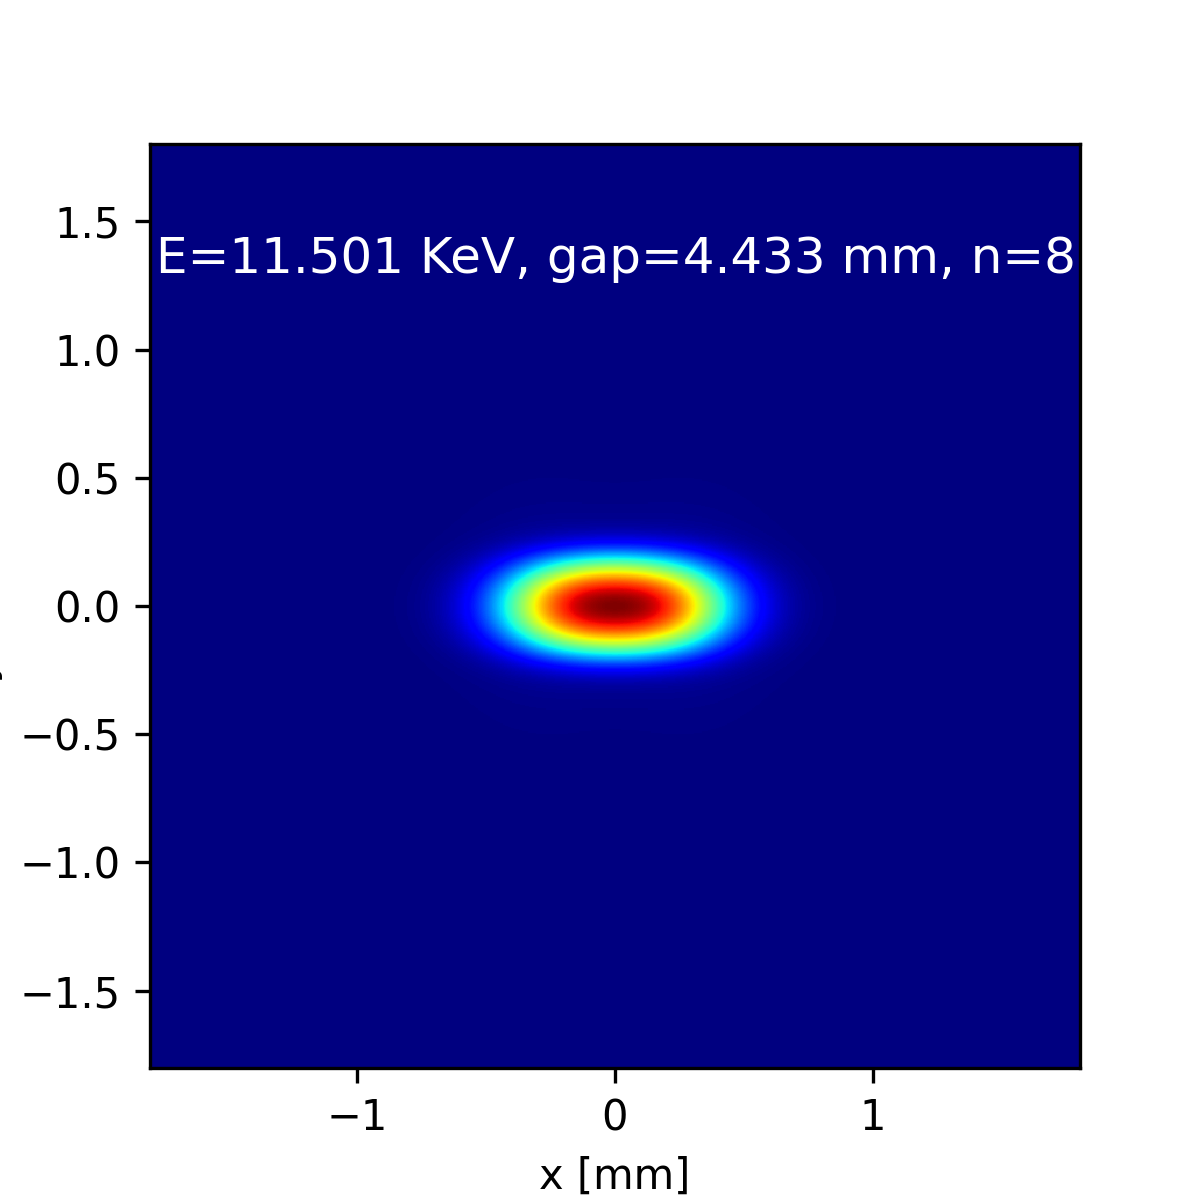
\includegraphics[width=1\linewidth, height=7cm]{photonbeam_right_E=11.501 KeV, gap=4.433 mm, n=8.png} 
\caption{Photon beam with perfectly aligned electron beam}
\end{subfigure}
\begin{subfigure}{0.4\textwidth}
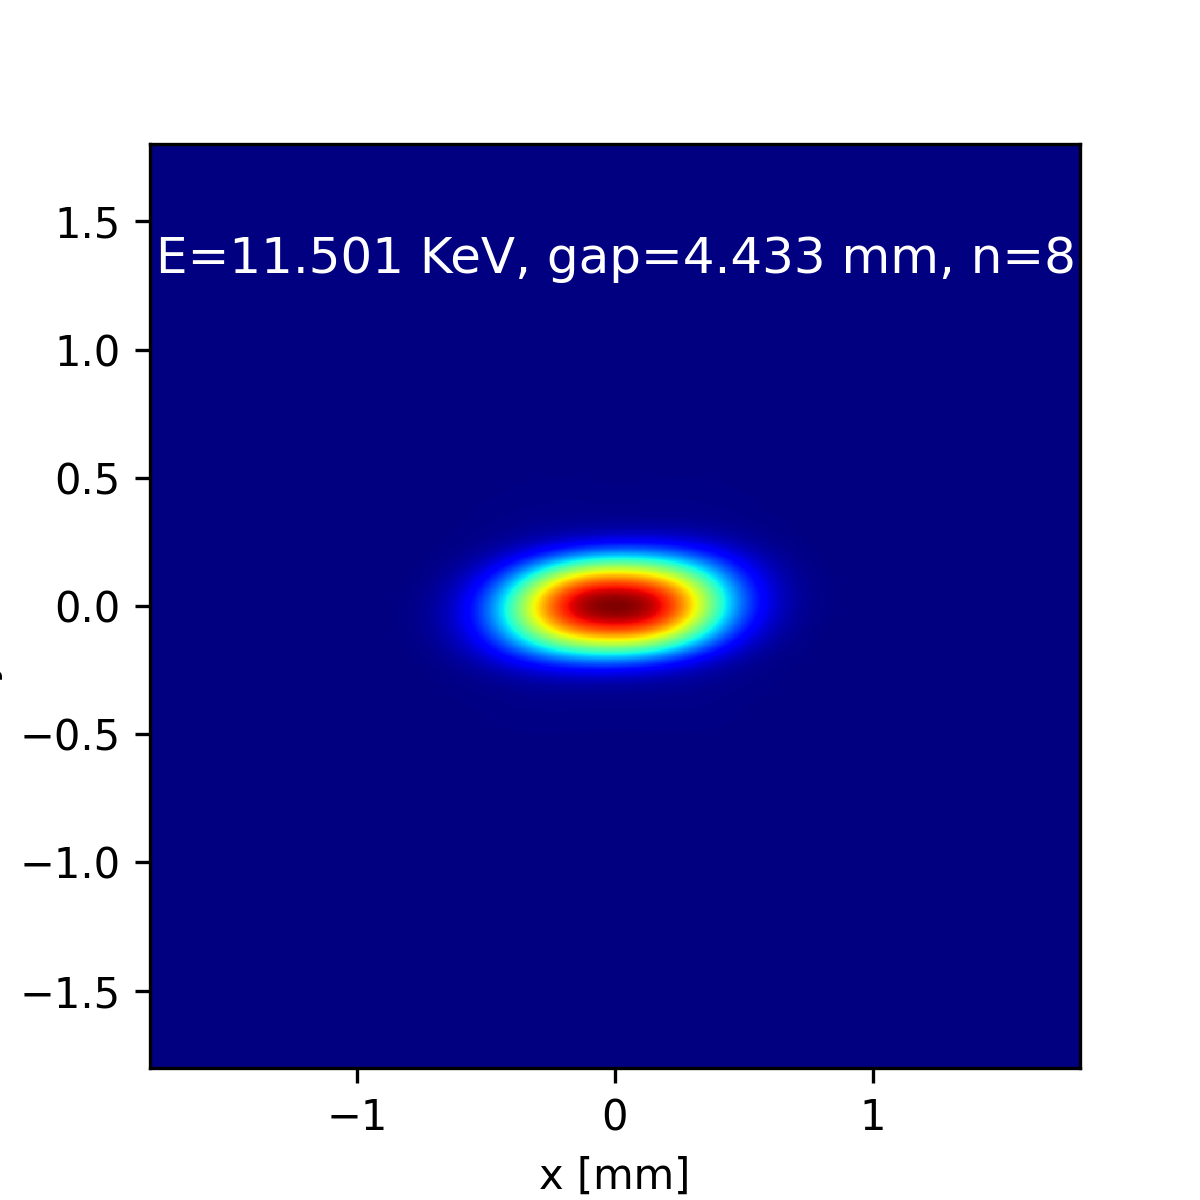
\includegraphics[width=1\linewidth, height=7cm]{photonbeam_tilted_E=11.501 KeV, gap=4.433 mm, n=8.png}
\caption{Photon beam with 2-degree electron beam tilt}
\end{subfigure}
\caption{Photon flux density distribution for different electron beam configurations at E = 11.501 KeV, gap = 4.433 mm, and n = 8.}
\label{fig:ressonance}
\end{figure}
            

\begin{figure}[H]
\centering
\begin{subfigure}{0.4\textwidth}
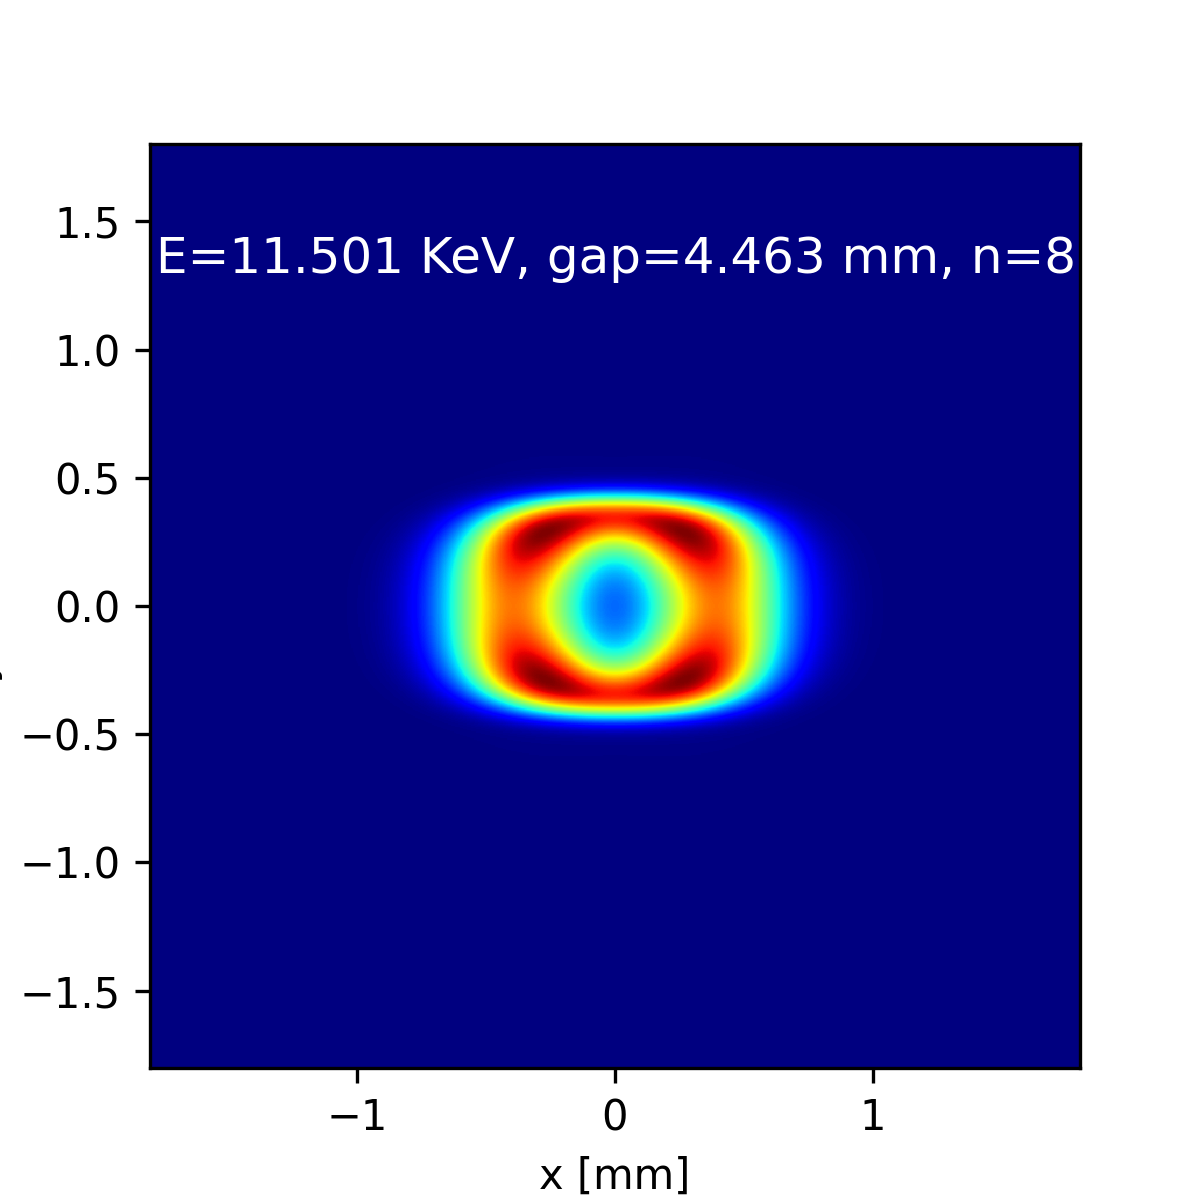
\includegraphics[width=1\linewidth, height=7cm]{photonbeam_right_E=11.501 KeV, gap=4.463 mm, n=8.png} 
\caption{Photon beam with perfectly aligned electron beam (gap = 4.463 mm)}
\end{subfigure}
\begin{subfigure}{0.4\textwidth}
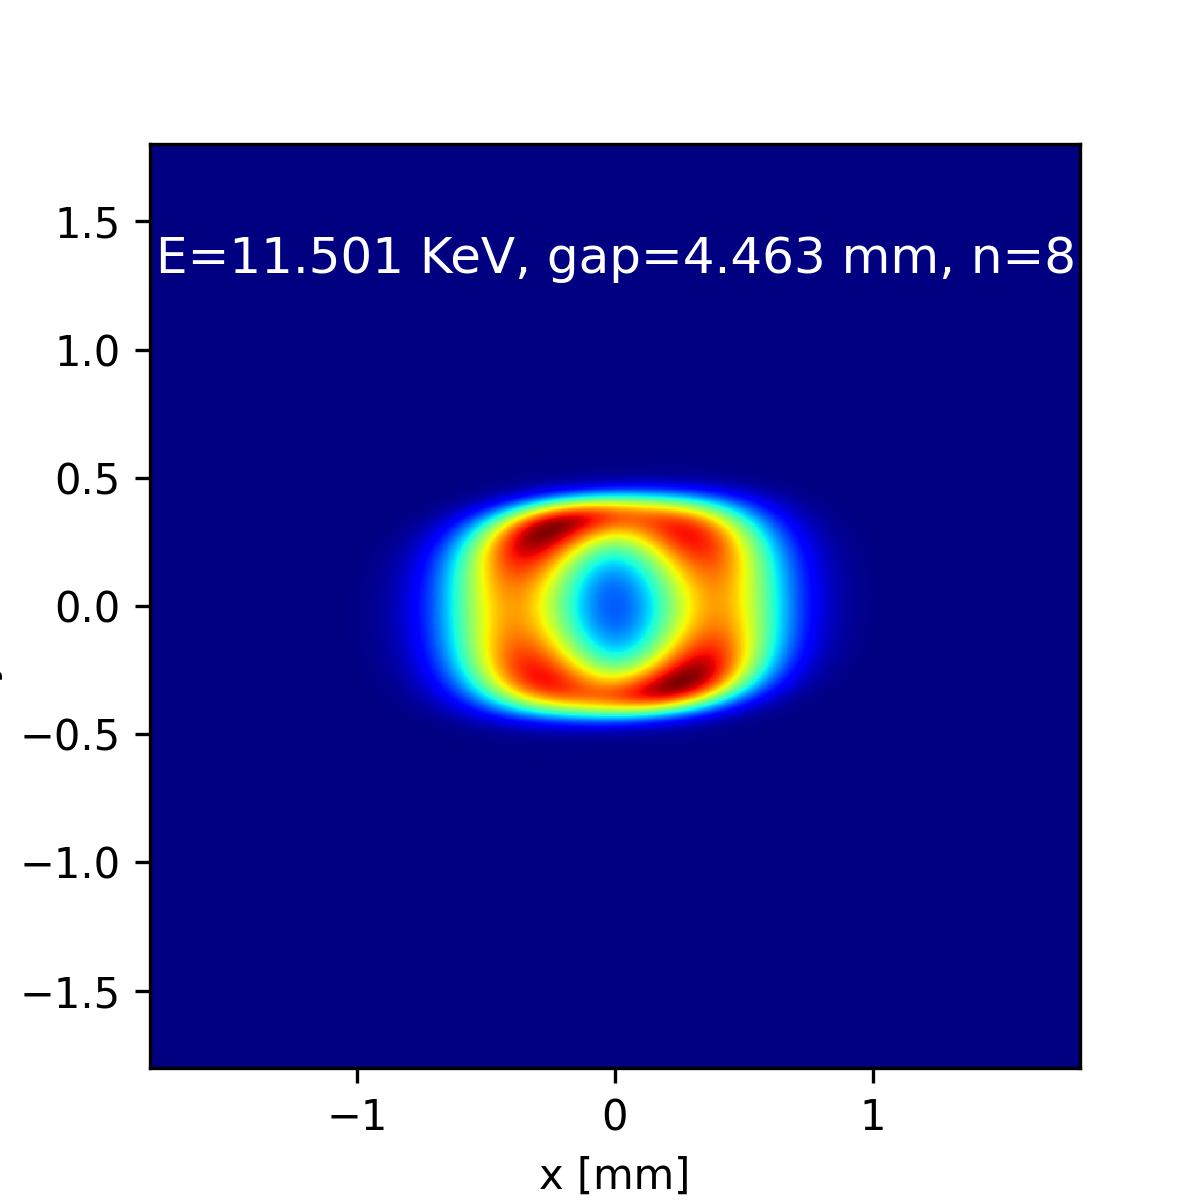
\includegraphics[width=1\linewidth, height=7cm]{photonbeam_tilted_E=11.501 KeV, gap=4.463 mm, n=8.png}
\caption{Photon beam with 4-degree electron beam tilt (gap = 4.463 mm)}
\end{subfigure}
\caption{Photon flux density distribution at E = 11.501 KeV and n = 8 for gap = 4.463 mm.}
\label{fig:pt2}
\end{figure}
    
\begin{figure}[H]
\centering
\begin{subfigure}{0.4\textwidth}
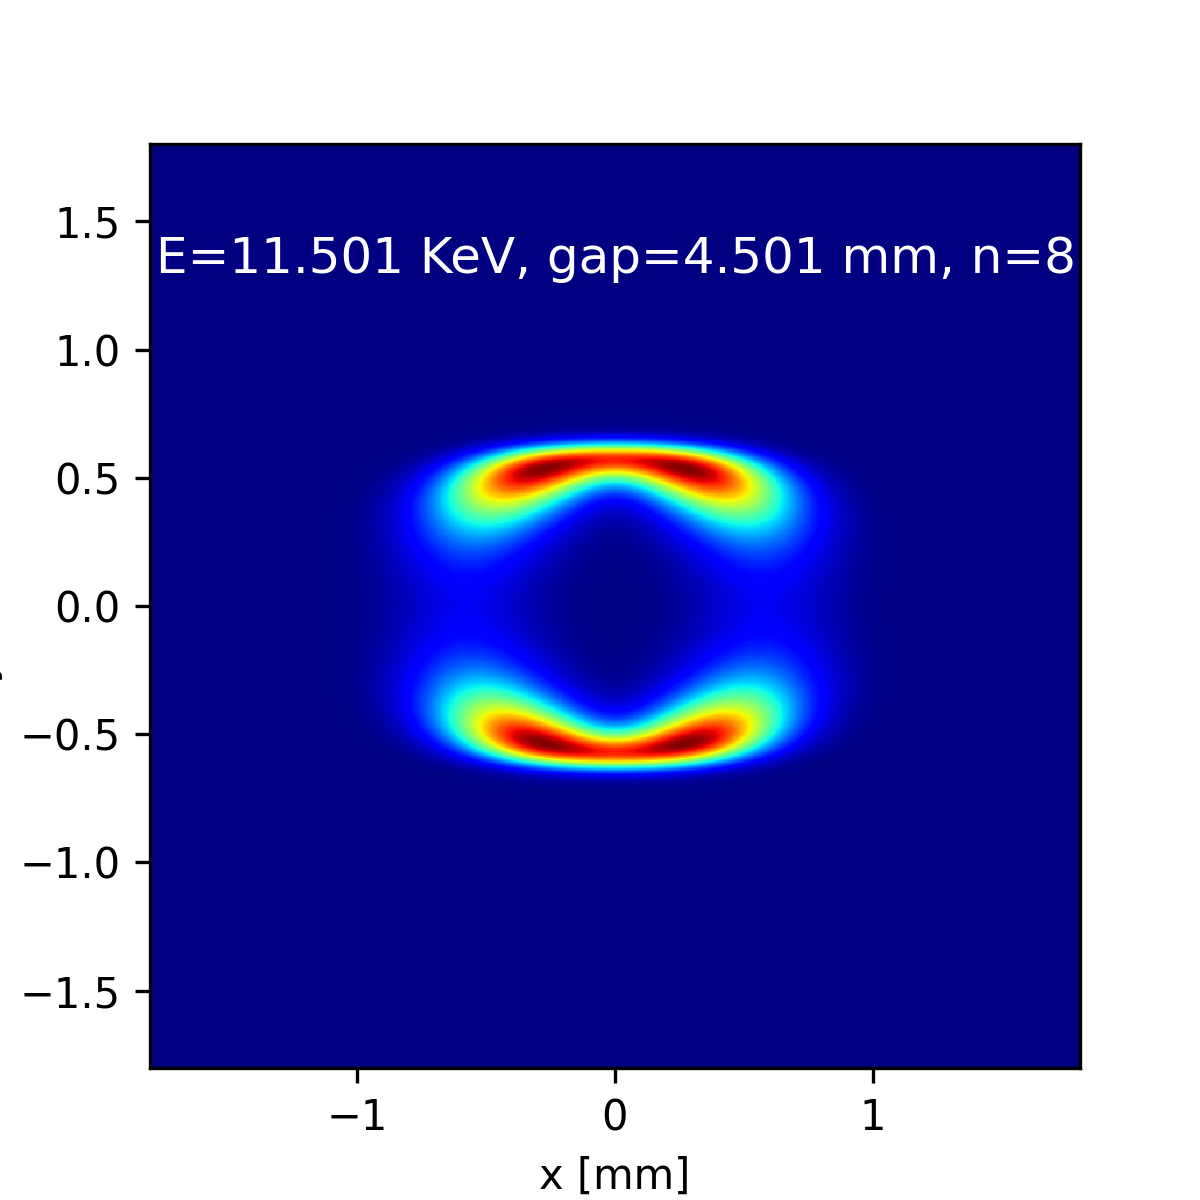
\includegraphics[width=1\linewidth, height=7cm]{photonbeam_right_E=11.501 KeV, gap=4.501 mm, n=8.png} 
\caption{Photon beam with perfectly aligned electron beam (gap = 4.501 mm)}
\end{subfigure}
\begin{subfigure}{0.4\textwidth}
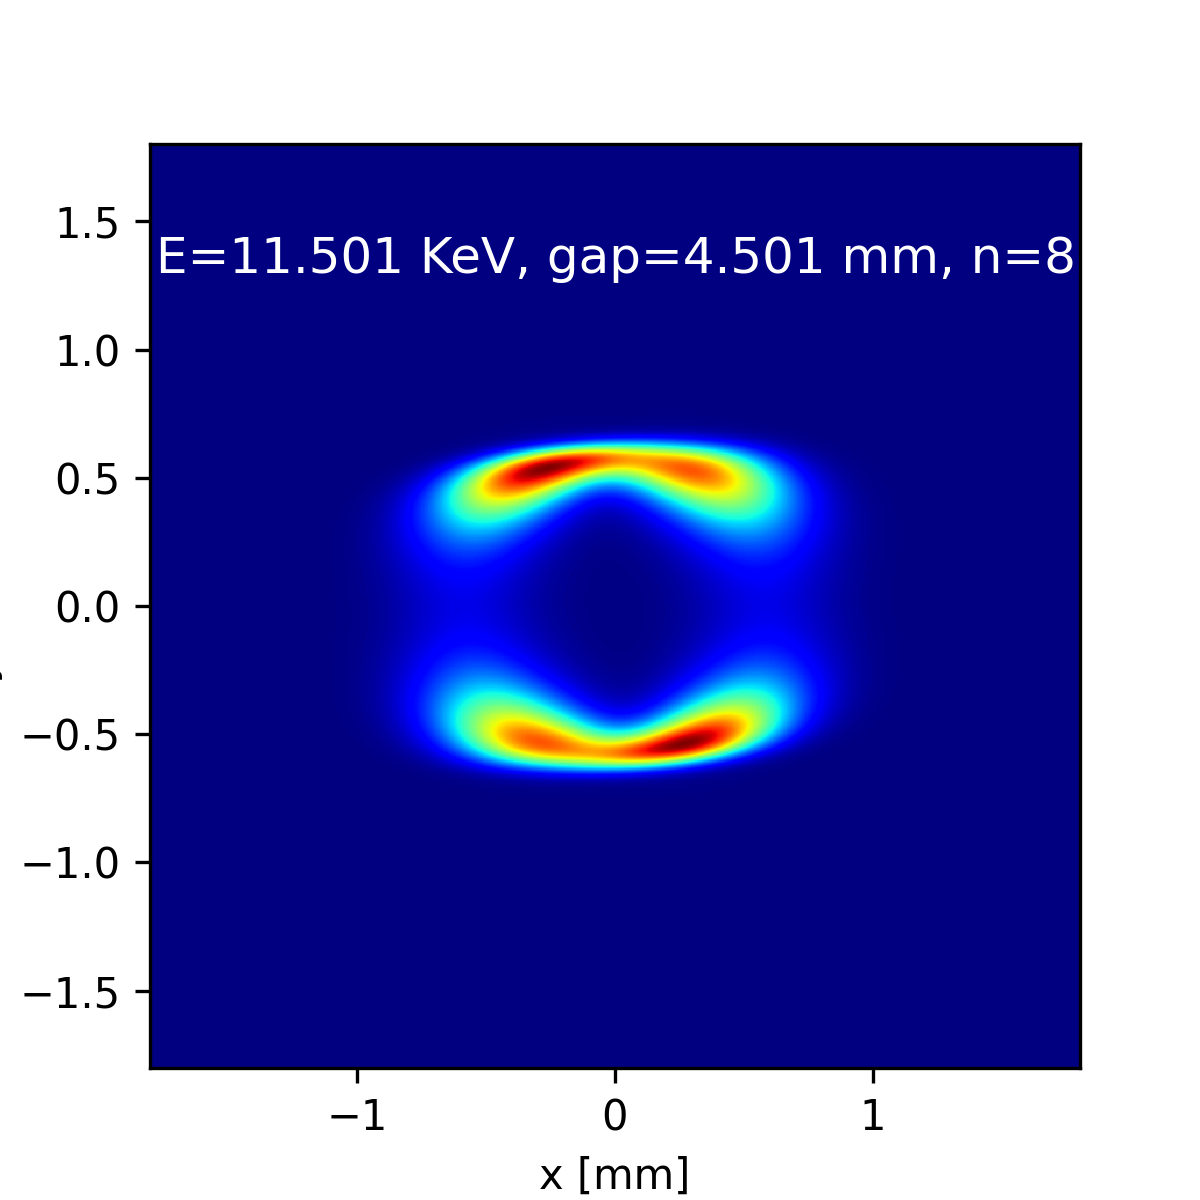
\includegraphics[width=1\linewidth, height=7cm]{photonbeam_tilted_E=11.501 KeV, gap=4.501 mm, n=8.png}
\caption{Photon beam with 4-degree electron beam tilt (gap = 4.501 mm)}
\end{subfigure}
\caption{Photon flux density distribution at E = 11.501 KeV and n = 8 for gap = 4.501 mm.}
\label{fig:pt3}
\end{figure}

The figures above demonstrate
 that when the electron beam is tilted,
  the photon beam flux density loses its
   symmetry during detuning. This was the objective of the experiment:
    to alter the energy of the emitted photons by adjusting
     the undulator gap, record the corresponding spatial distribution of the flux and analyze the distribution.

\section{Experiment}

Figures \ref{fig:meas_pt1,fig:meas_pt2,fig:meas_pt3,fig:meas_pt4}  present flux density distributions measured
 at various undulator gap settings. Notably, an asymmetry
  in the flux distribution becomes apparent when the
   undulator is detuned, particularly at the last two
    gap settings ($4.496$ mm and $4.511$ mm). According to simulations,
     this asymmetry suggests the presence of an electron beam tilt
      in this straight section of the storage ring.

\begin{figure}[H]
\centering
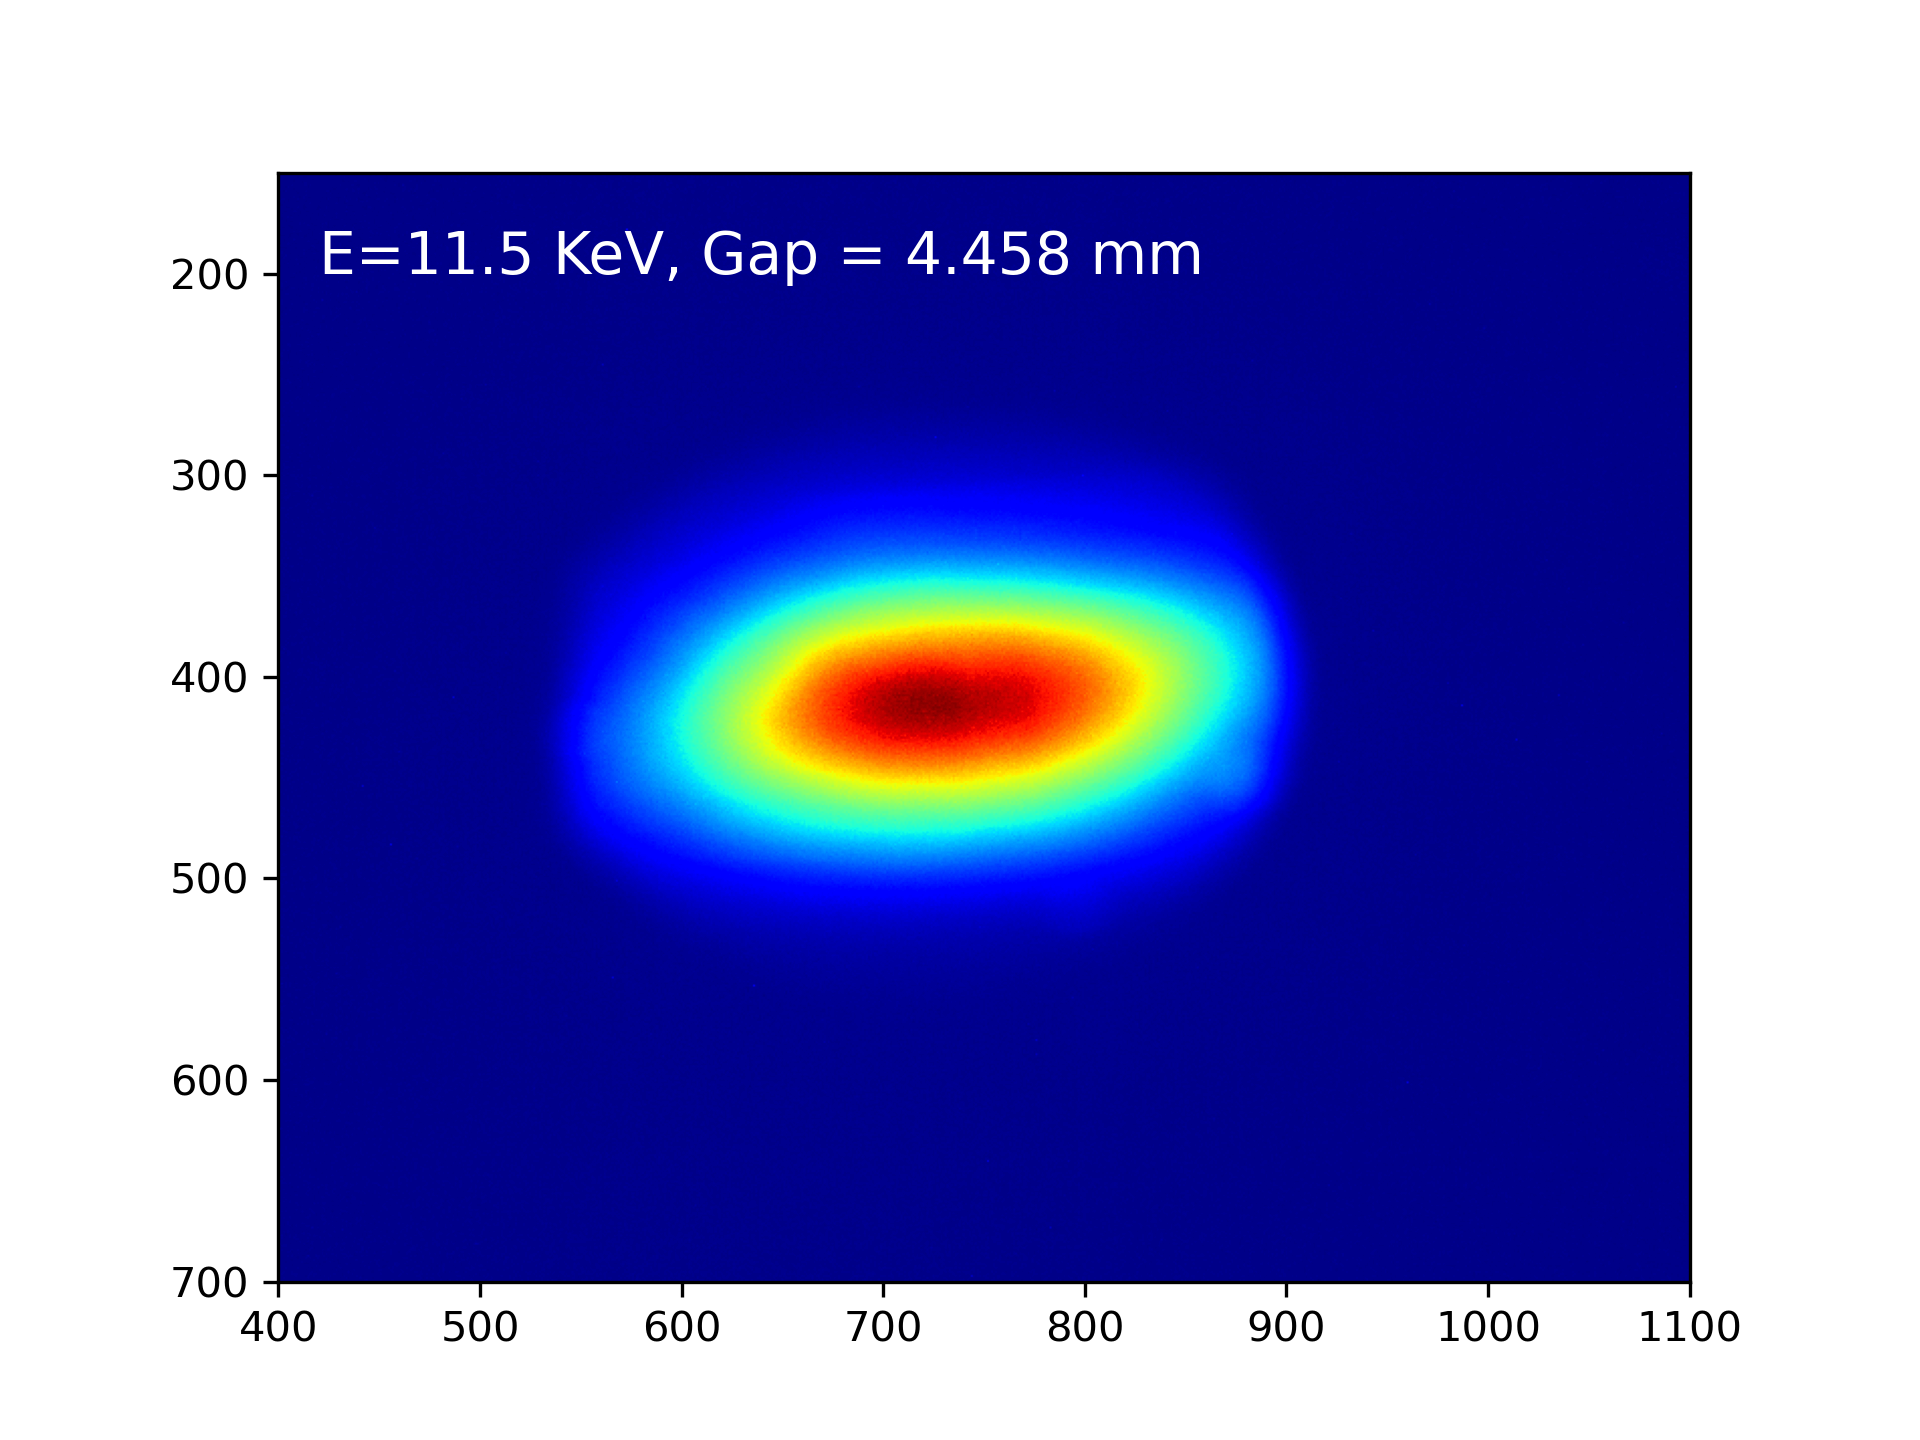
\includegraphics[width=0.5\textwidth]{images_E11500eV_G4.458mm.png}
\caption{Measured flux density distribution for gap $4.458$ mm}
\label{fig:meas_pt1}
\end{figure}

\begin{figure}[H]
\centering
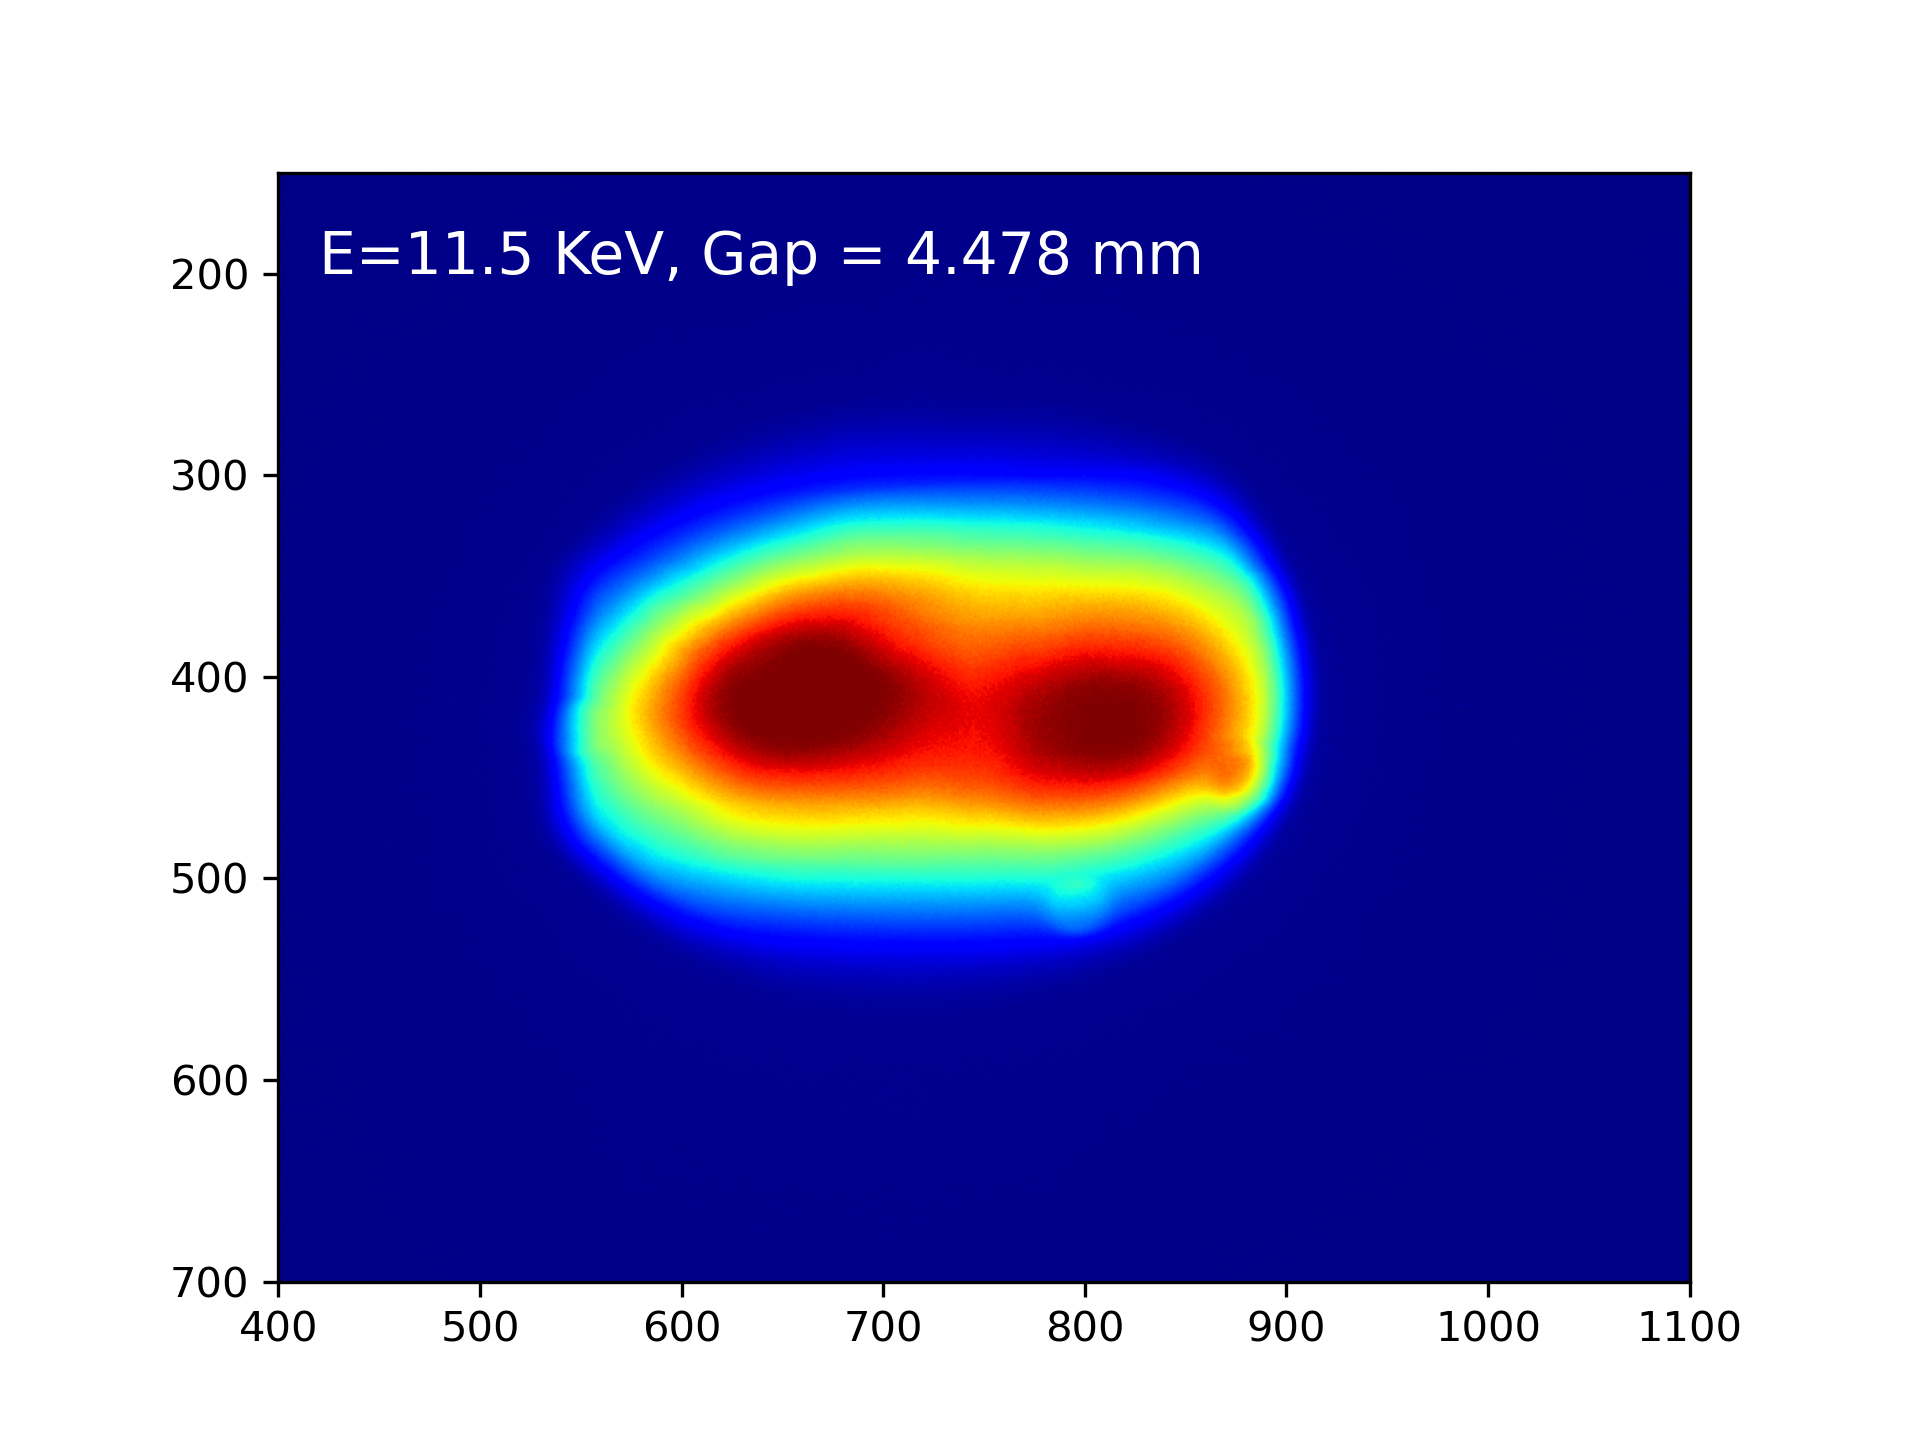
\includegraphics[width=0.5\textwidth]{images_E11500eV_G4.478mm.png}
\caption{Measured flux density distribution for gap $4.478$ mm}
\label{fig:meas_pt2}
\end{figure}

\begin{figure}[H]
\centering
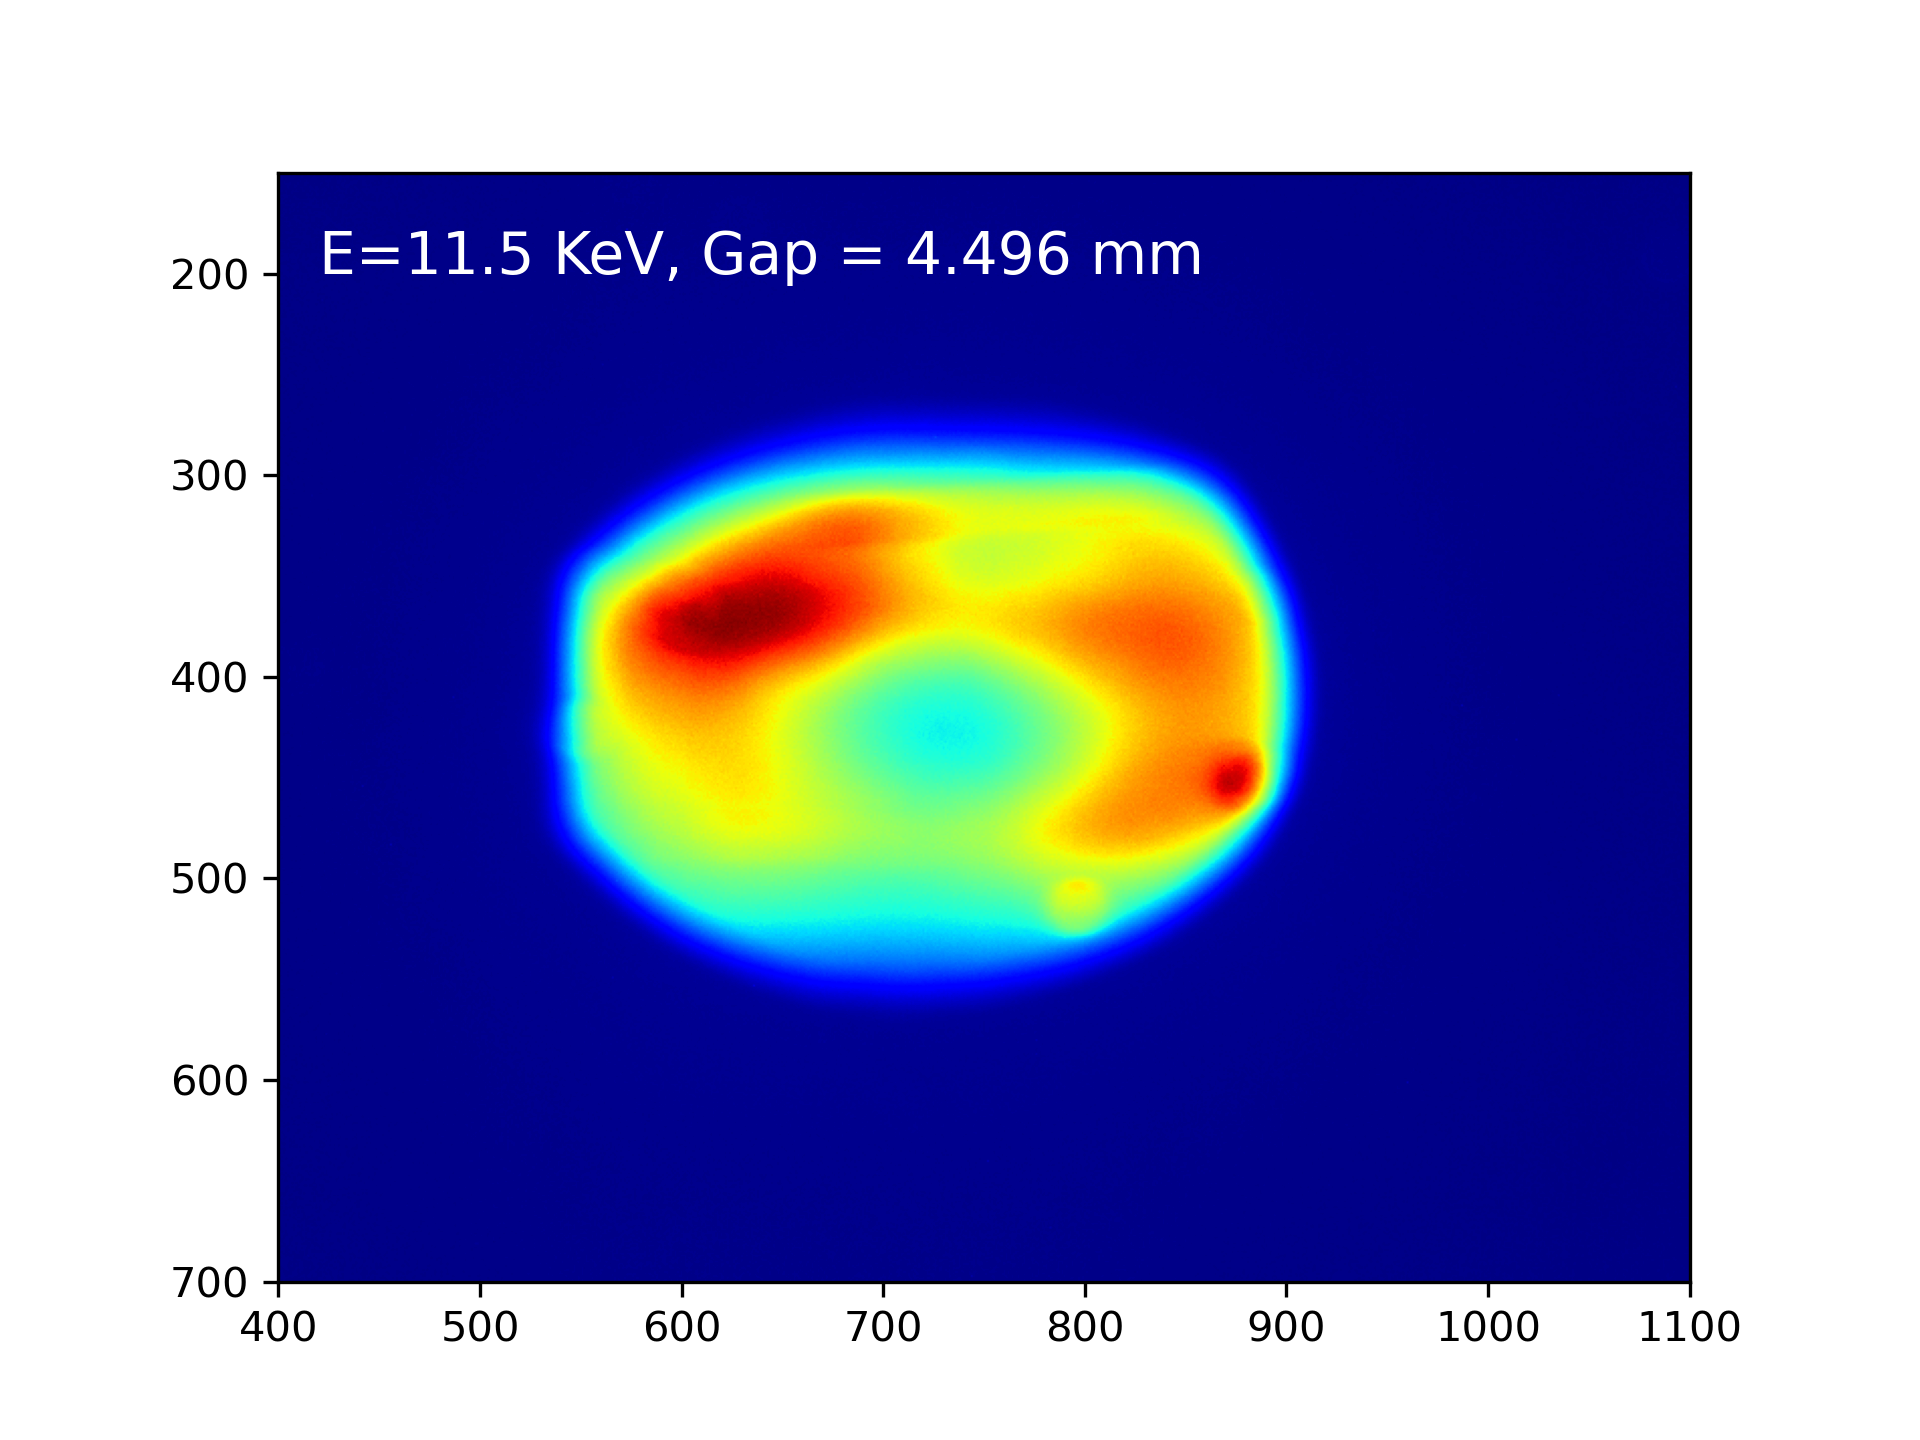
\includegraphics[width=0.5\textwidth]{images_E11500eV_G4.496mm.png}
\caption{Measured flux density distribution for gap $4.496$ mm}
\label{fig:meas_pt3}
\end{figure}

\begin{figure}[H]
\centering
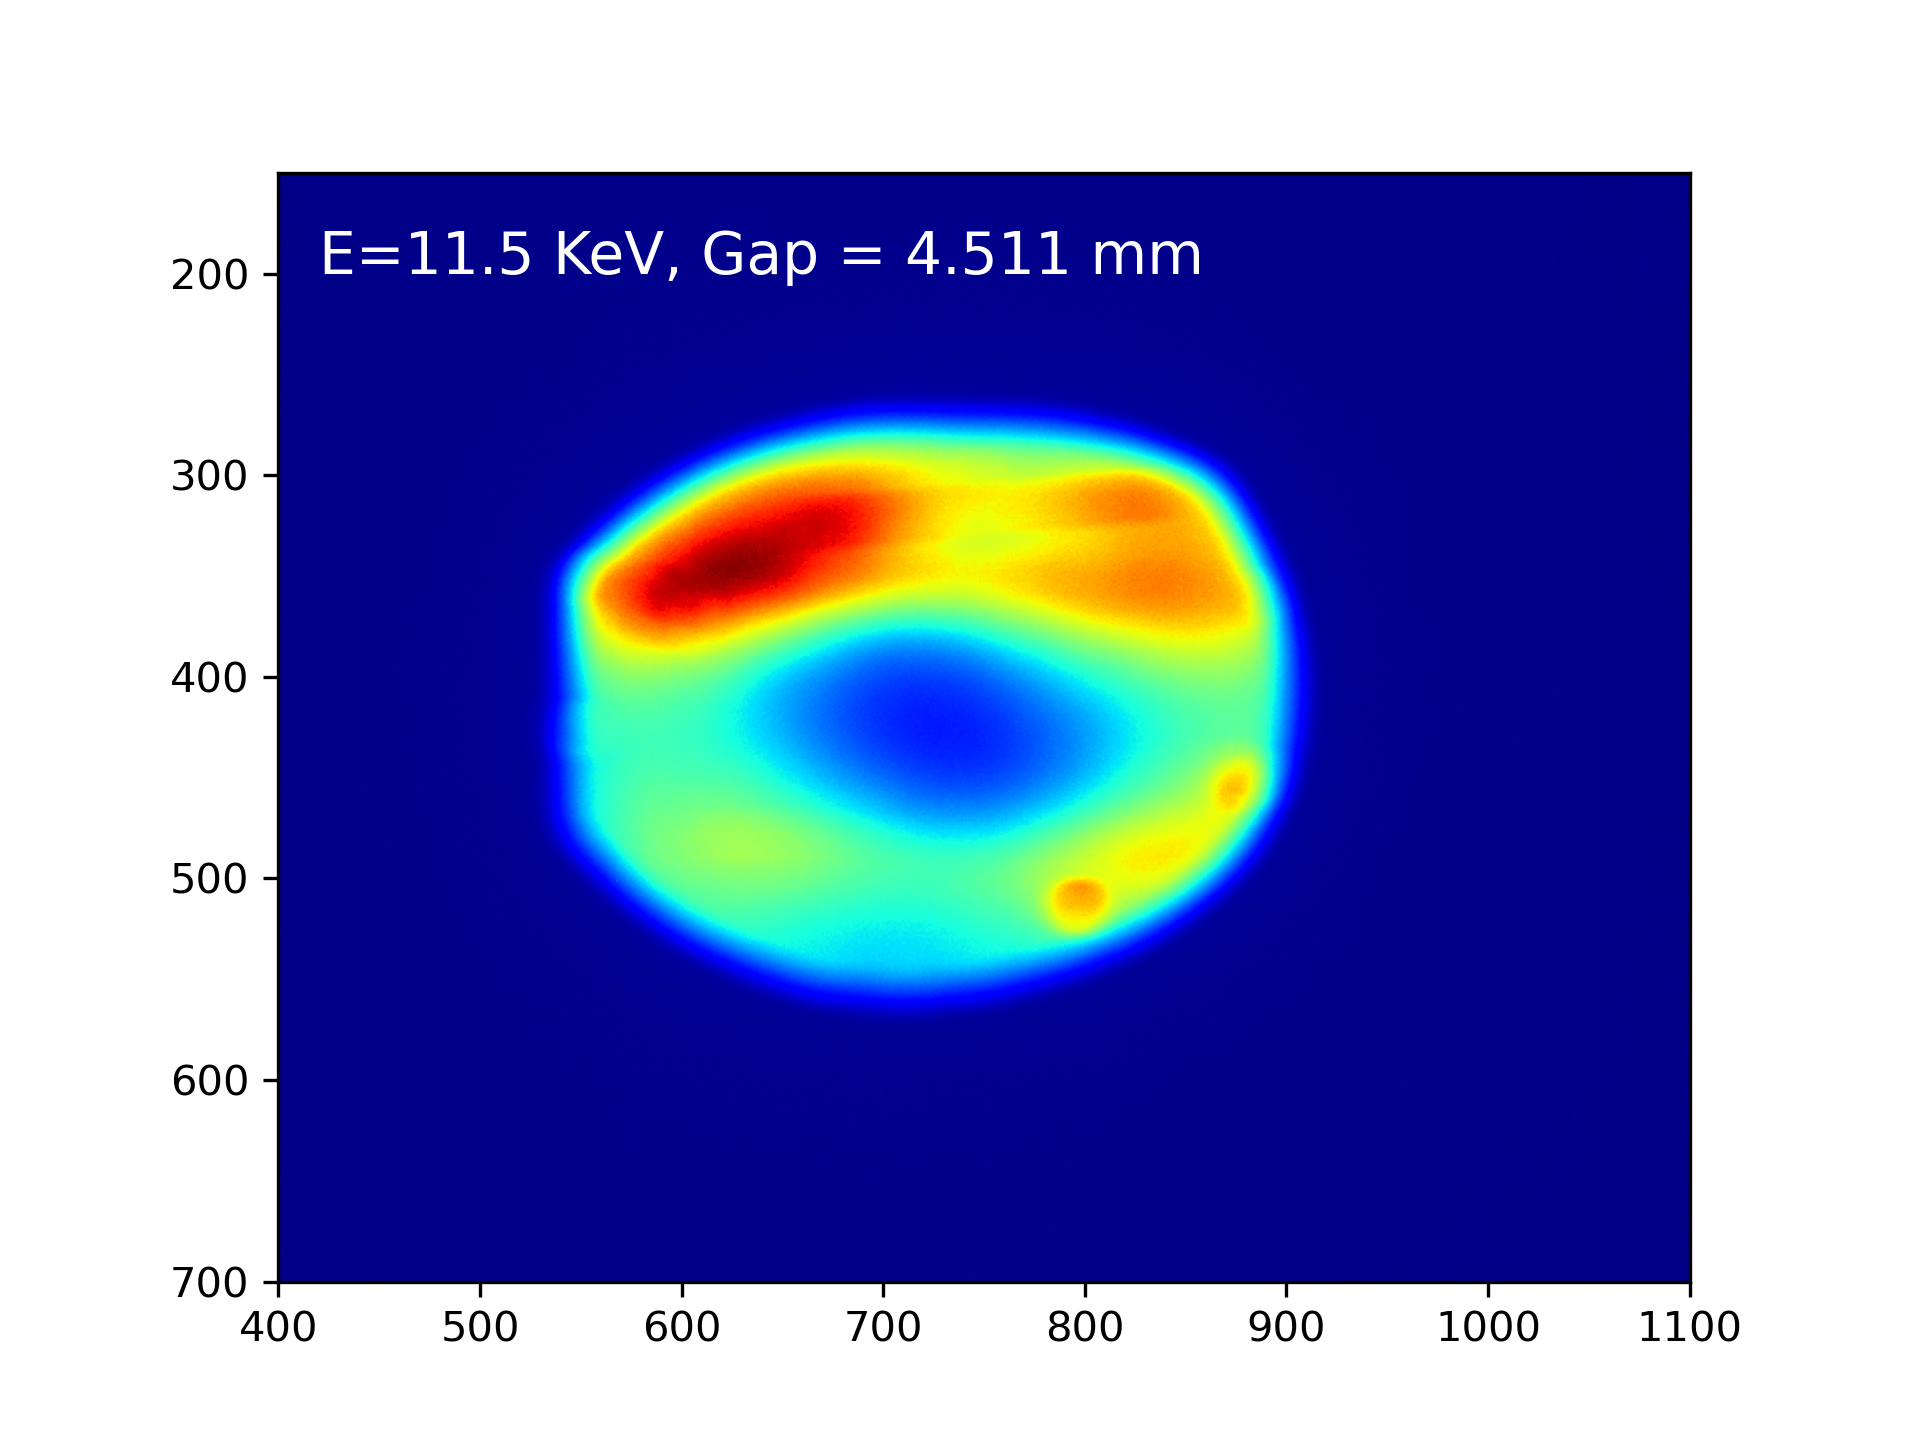
\includegraphics[width=0.5\textwidth]{images_E11500eV_G4.511mm.png}
\caption{Measured flux density distribution for gap $4.511$ mm}
\label{fig:meas_pt4}
\end{figure}

To verify the hypothesis of an electron beam tilt,
 an attempt was made to correct the tilt by adjusting
  the machine's skew quadrupoles. The first step involved
   estimating the tilt using a fitted model of the storage ring,
    based on the most recent orbit response matrix. The fitting
     was performed using LOCO. A set of skew quadrupole adjustments 
     that corrected the beam tilt in the PAINEIRA straight section
      was identified. This correction can be seen in the figure below:
       the image on the left shows the electron beam distribution after
        fitting but without skew correction, while the image on the right
         shows the distribution after applying the skew correction.

\begin{figure}[H]
\centering
\begin{subfigure}{0.4\textwidth}
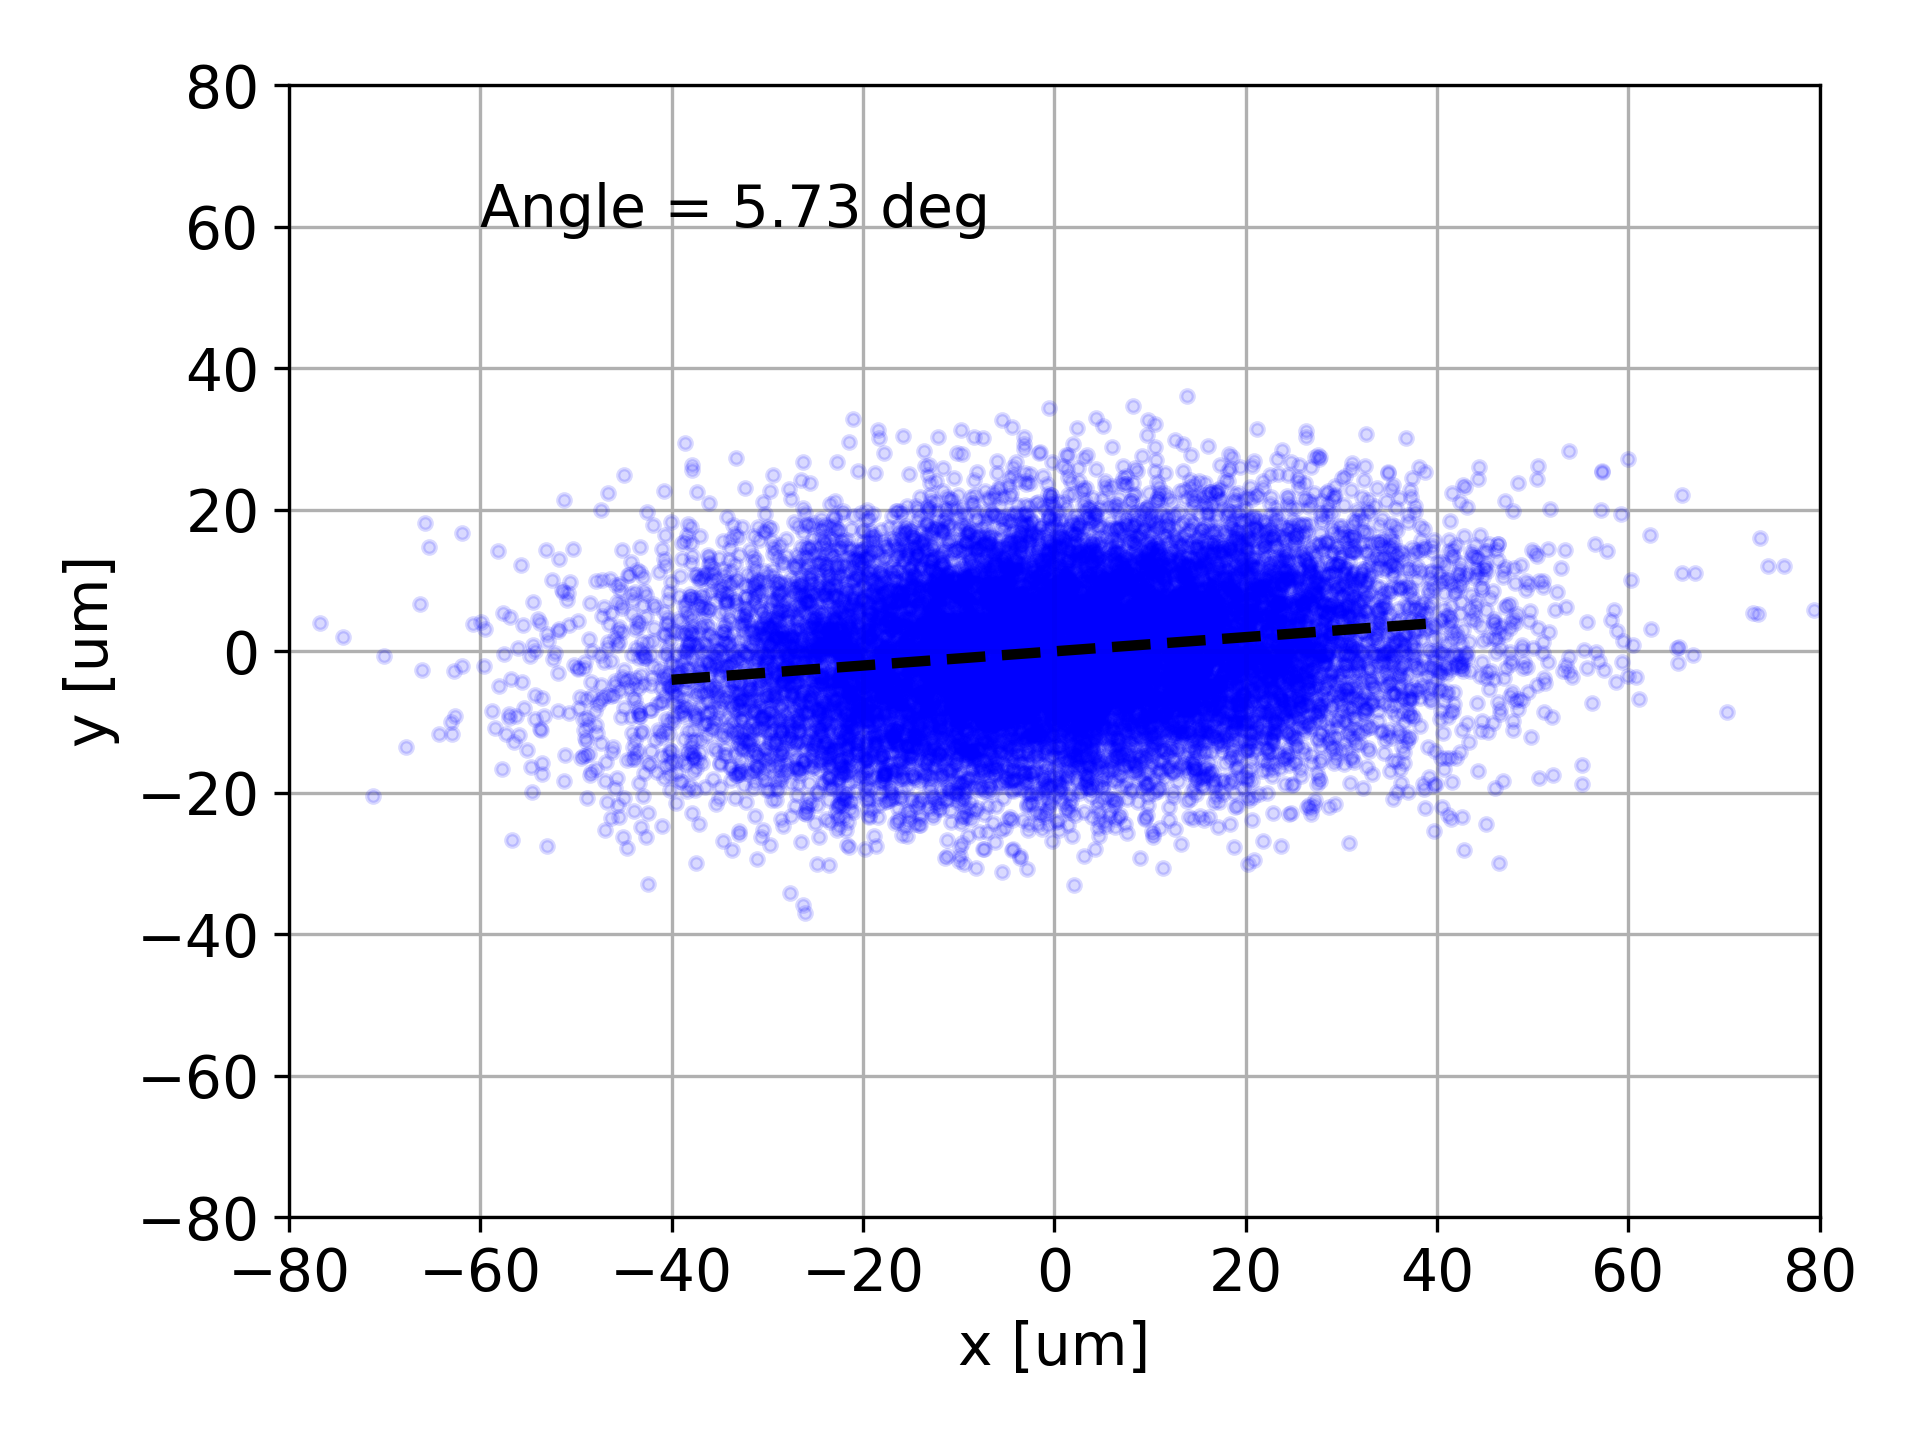
\includegraphics[width=1\linewidth, height=7cm]{ebeam_tilted.png} 
\caption{Electron beam distribution without skew correction}
\end{subfigure}
\begin{subfigure}{0.4\textwidth}
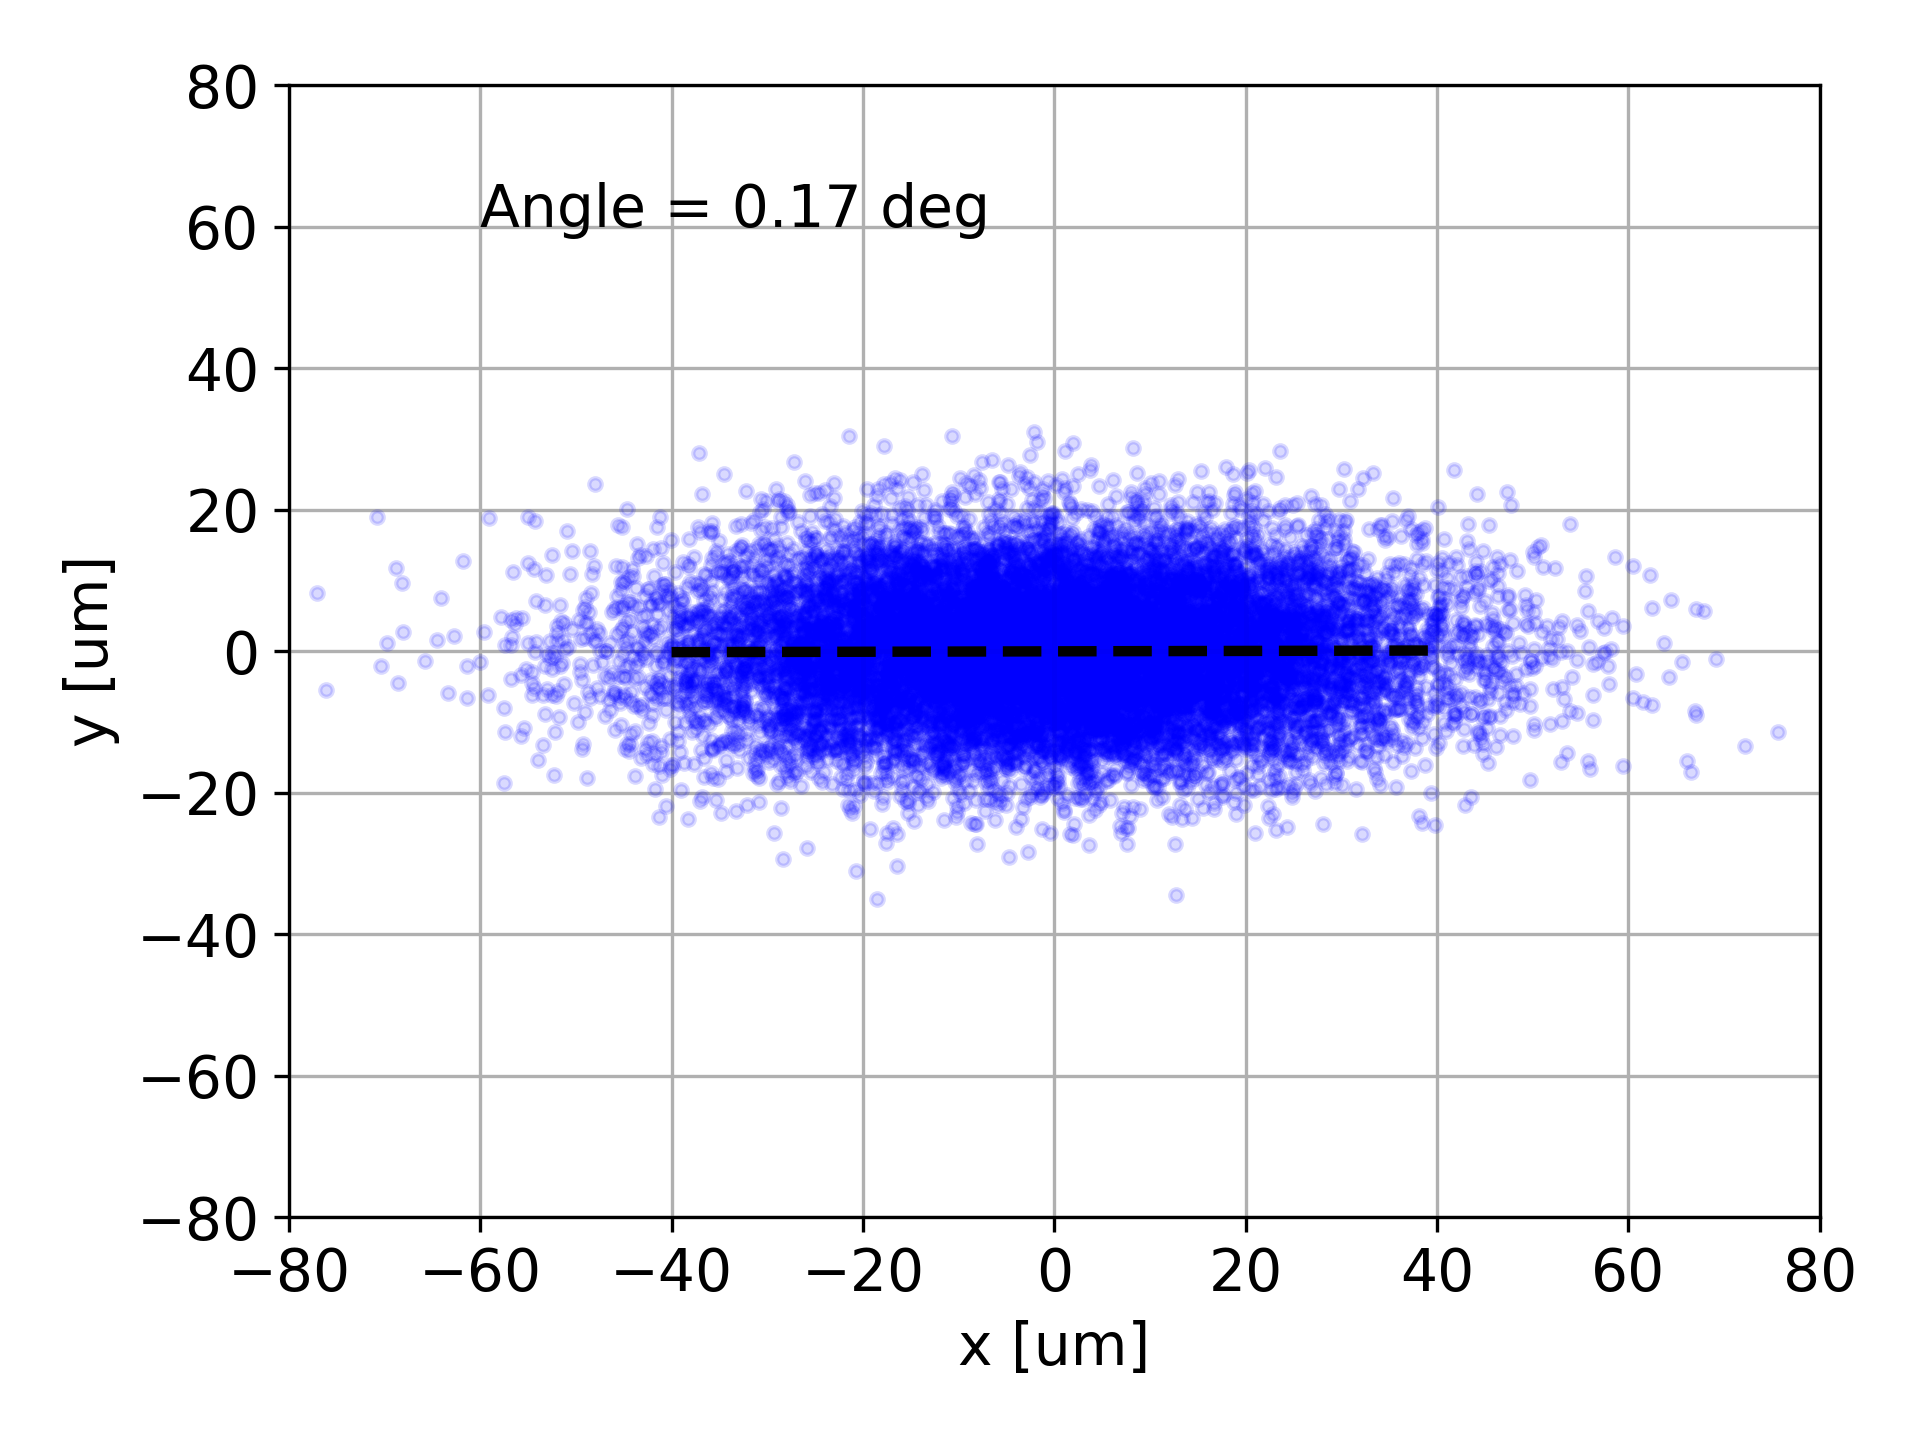
\includegraphics[width=1\linewidth, height=7cm]{ebeam_corrected.png}
\caption{Electron beam distribution with skew correction}
\end{subfigure}
\label{fig:model_angle}
\end{figure}


The force variation of the skew quadrupoles is shown in Figure \ref{fig:skew_forces}.

\begin{figure}[H]
\centering
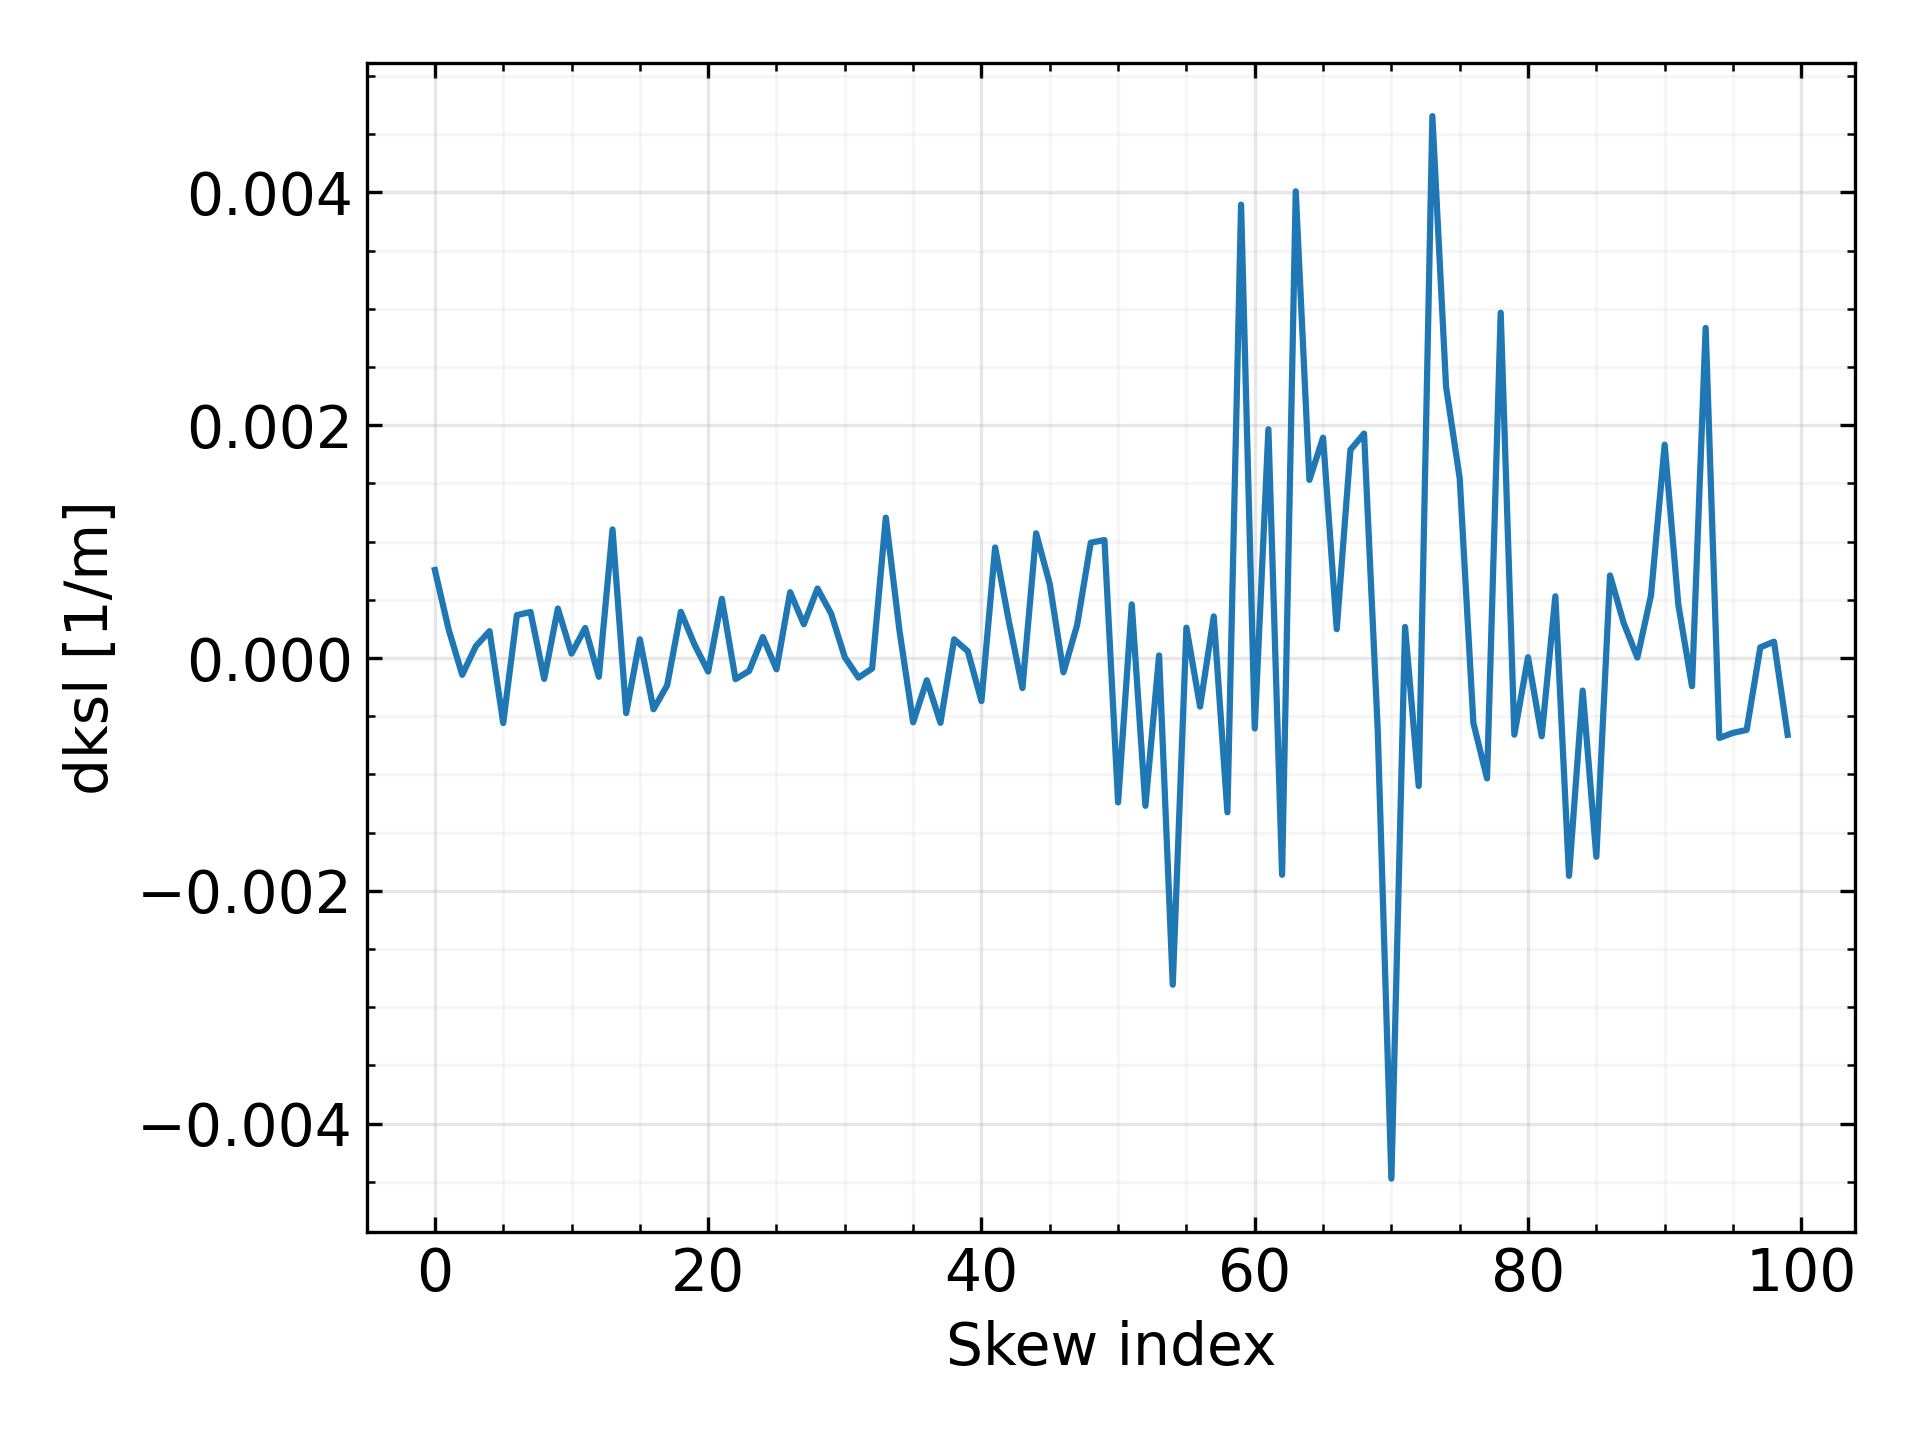
\includegraphics[width=0.5\textwidth]{dskl.png}
\caption{}
\label{fig:skew_forces}
\end{figure}


However, when the calculated skew adjustments
 were applied to the machine, no angle correction
  was observed in the beam as viewed on the DVF. Figures
   \ref{fig:meas_angle_1}-\ref{fig:meas_angle_2} illustrate the observed photon beam without skew correction,
    as well as after applying the full correction, double the correction
     strength, and quadruple the correction strength.

\begin{figure}[H]
\centering
\begin{subfigure}{0.4\textwidth}
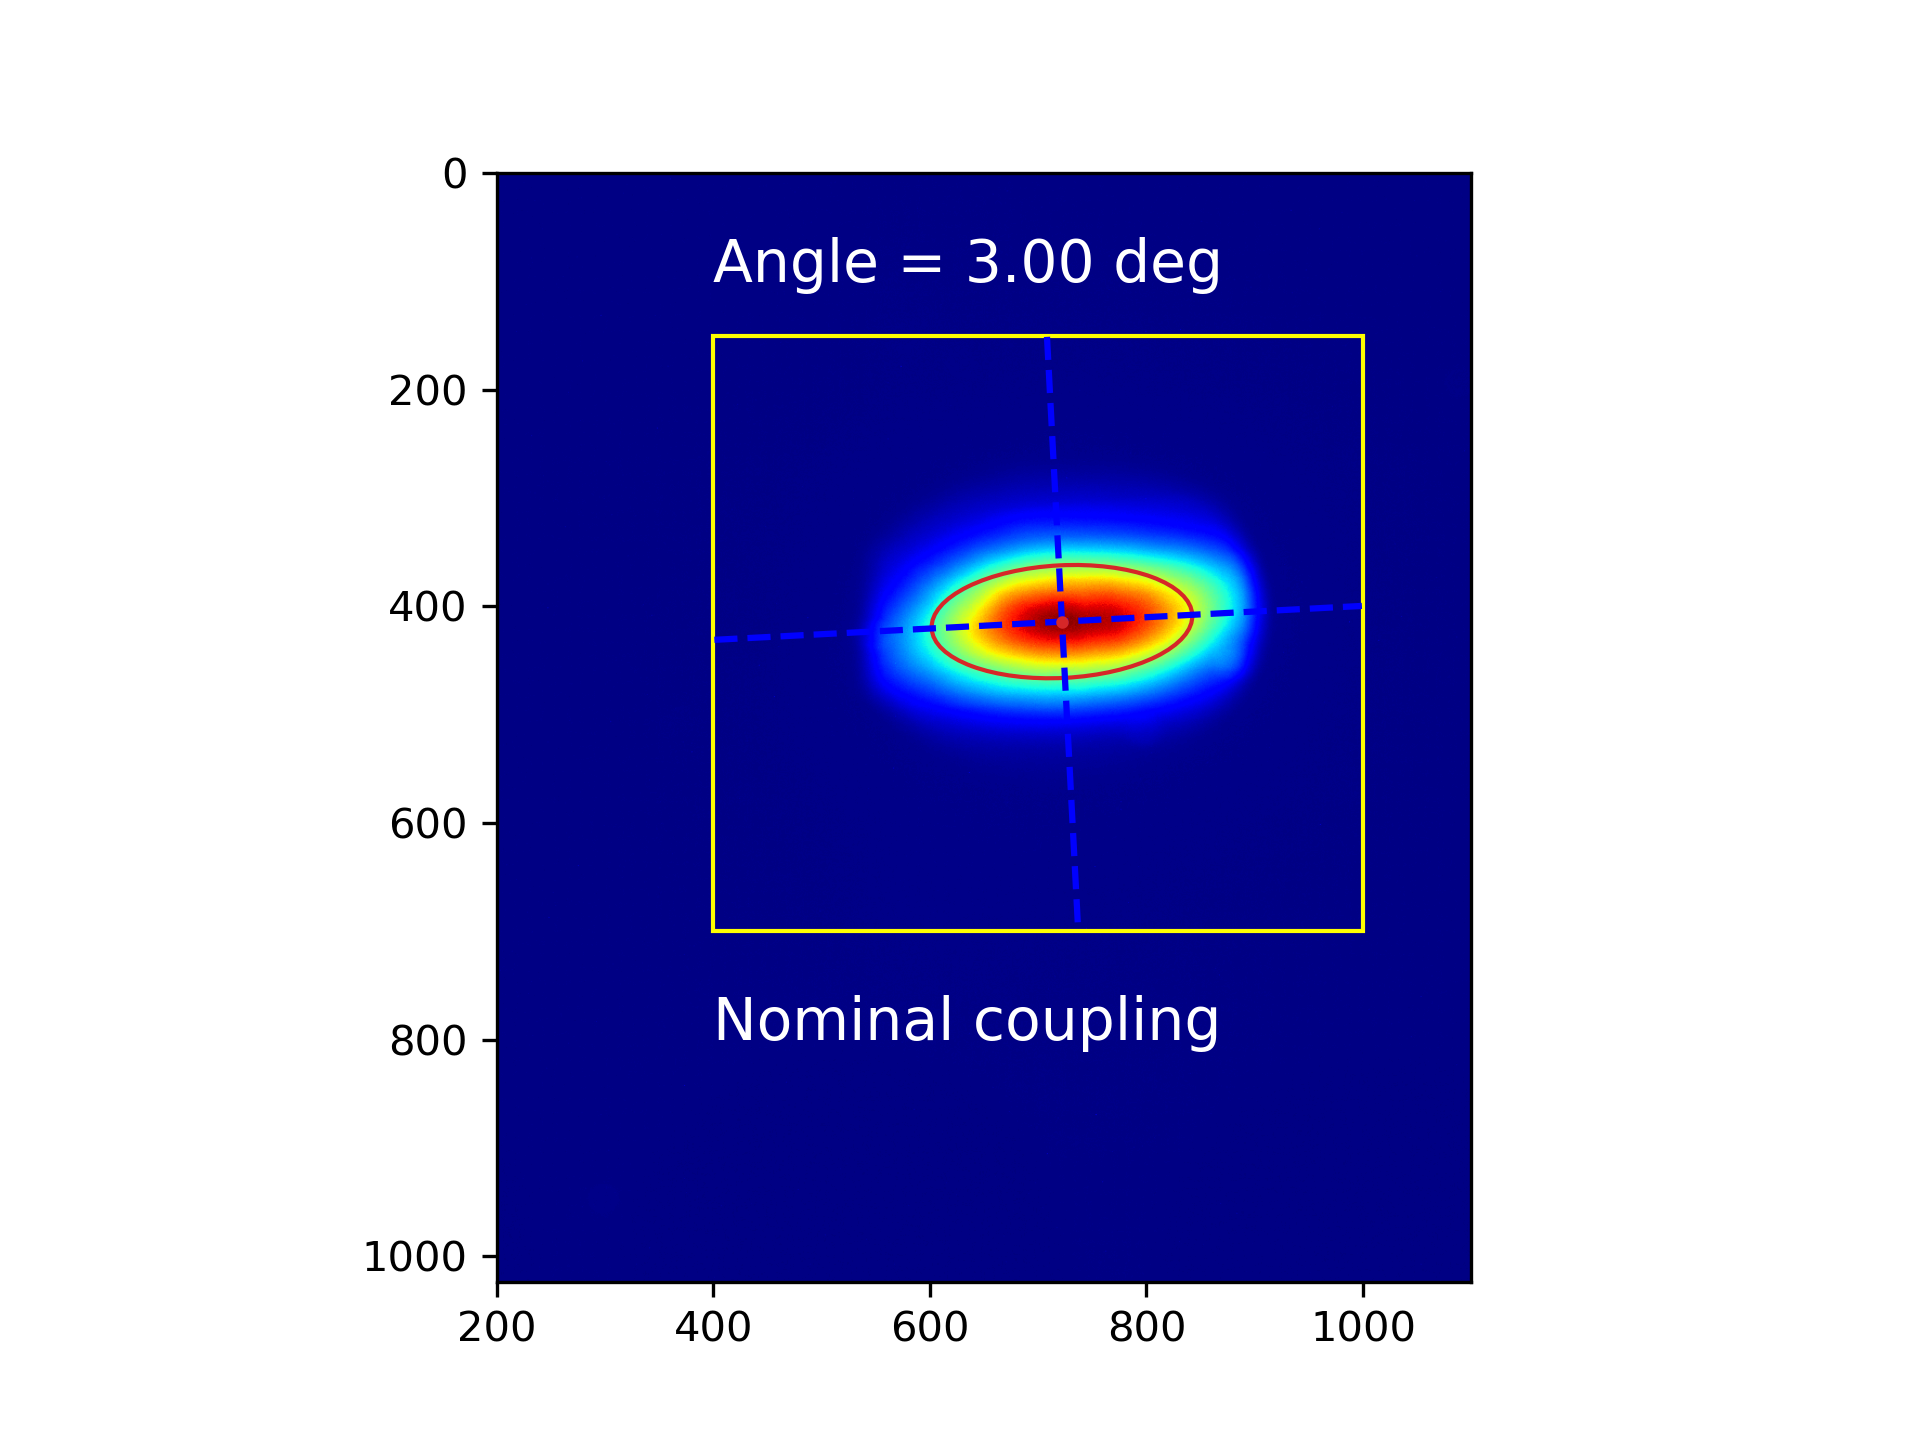
\includegraphics[width=1\linewidth, height=7cm]{Nominal_coupling_angle.png} 
\caption{Photon beam without skew correction}
\end{subfigure}
\begin{subfigure}{0.4\textwidth}
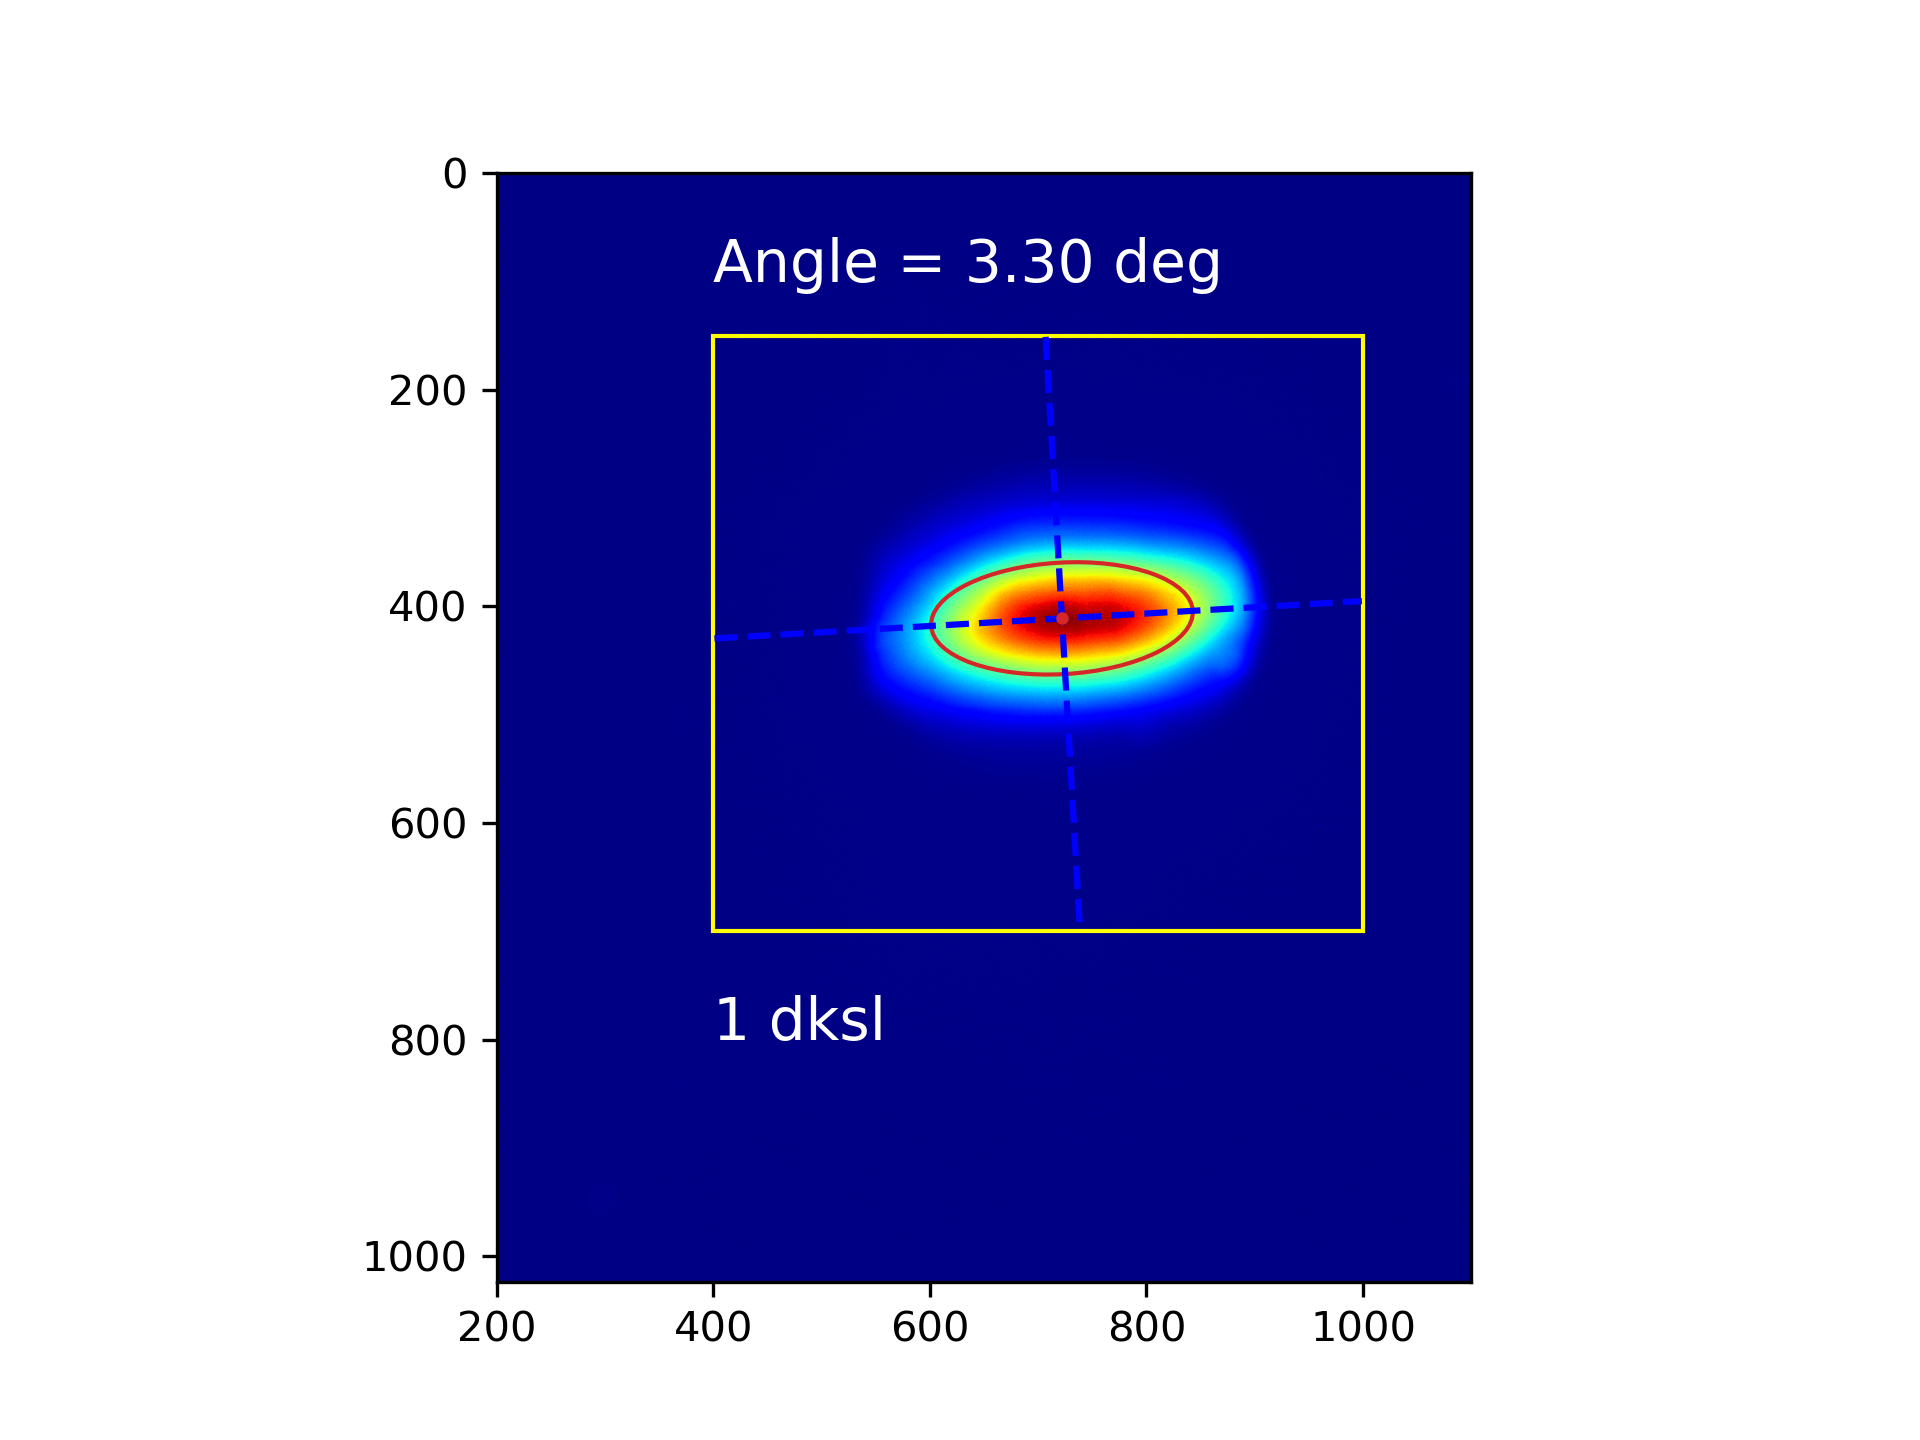
\includegraphics[width=1\linewidth, height=7cm]{1dksl_coupling_angle.png}
\caption{Photon beam with full skew correction}
\end{subfigure}
\label{fig:meas_angle_1}
\end{figure}

\begin{figure}[H]
\centering
\begin{subfigure}{0.4\textwidth}
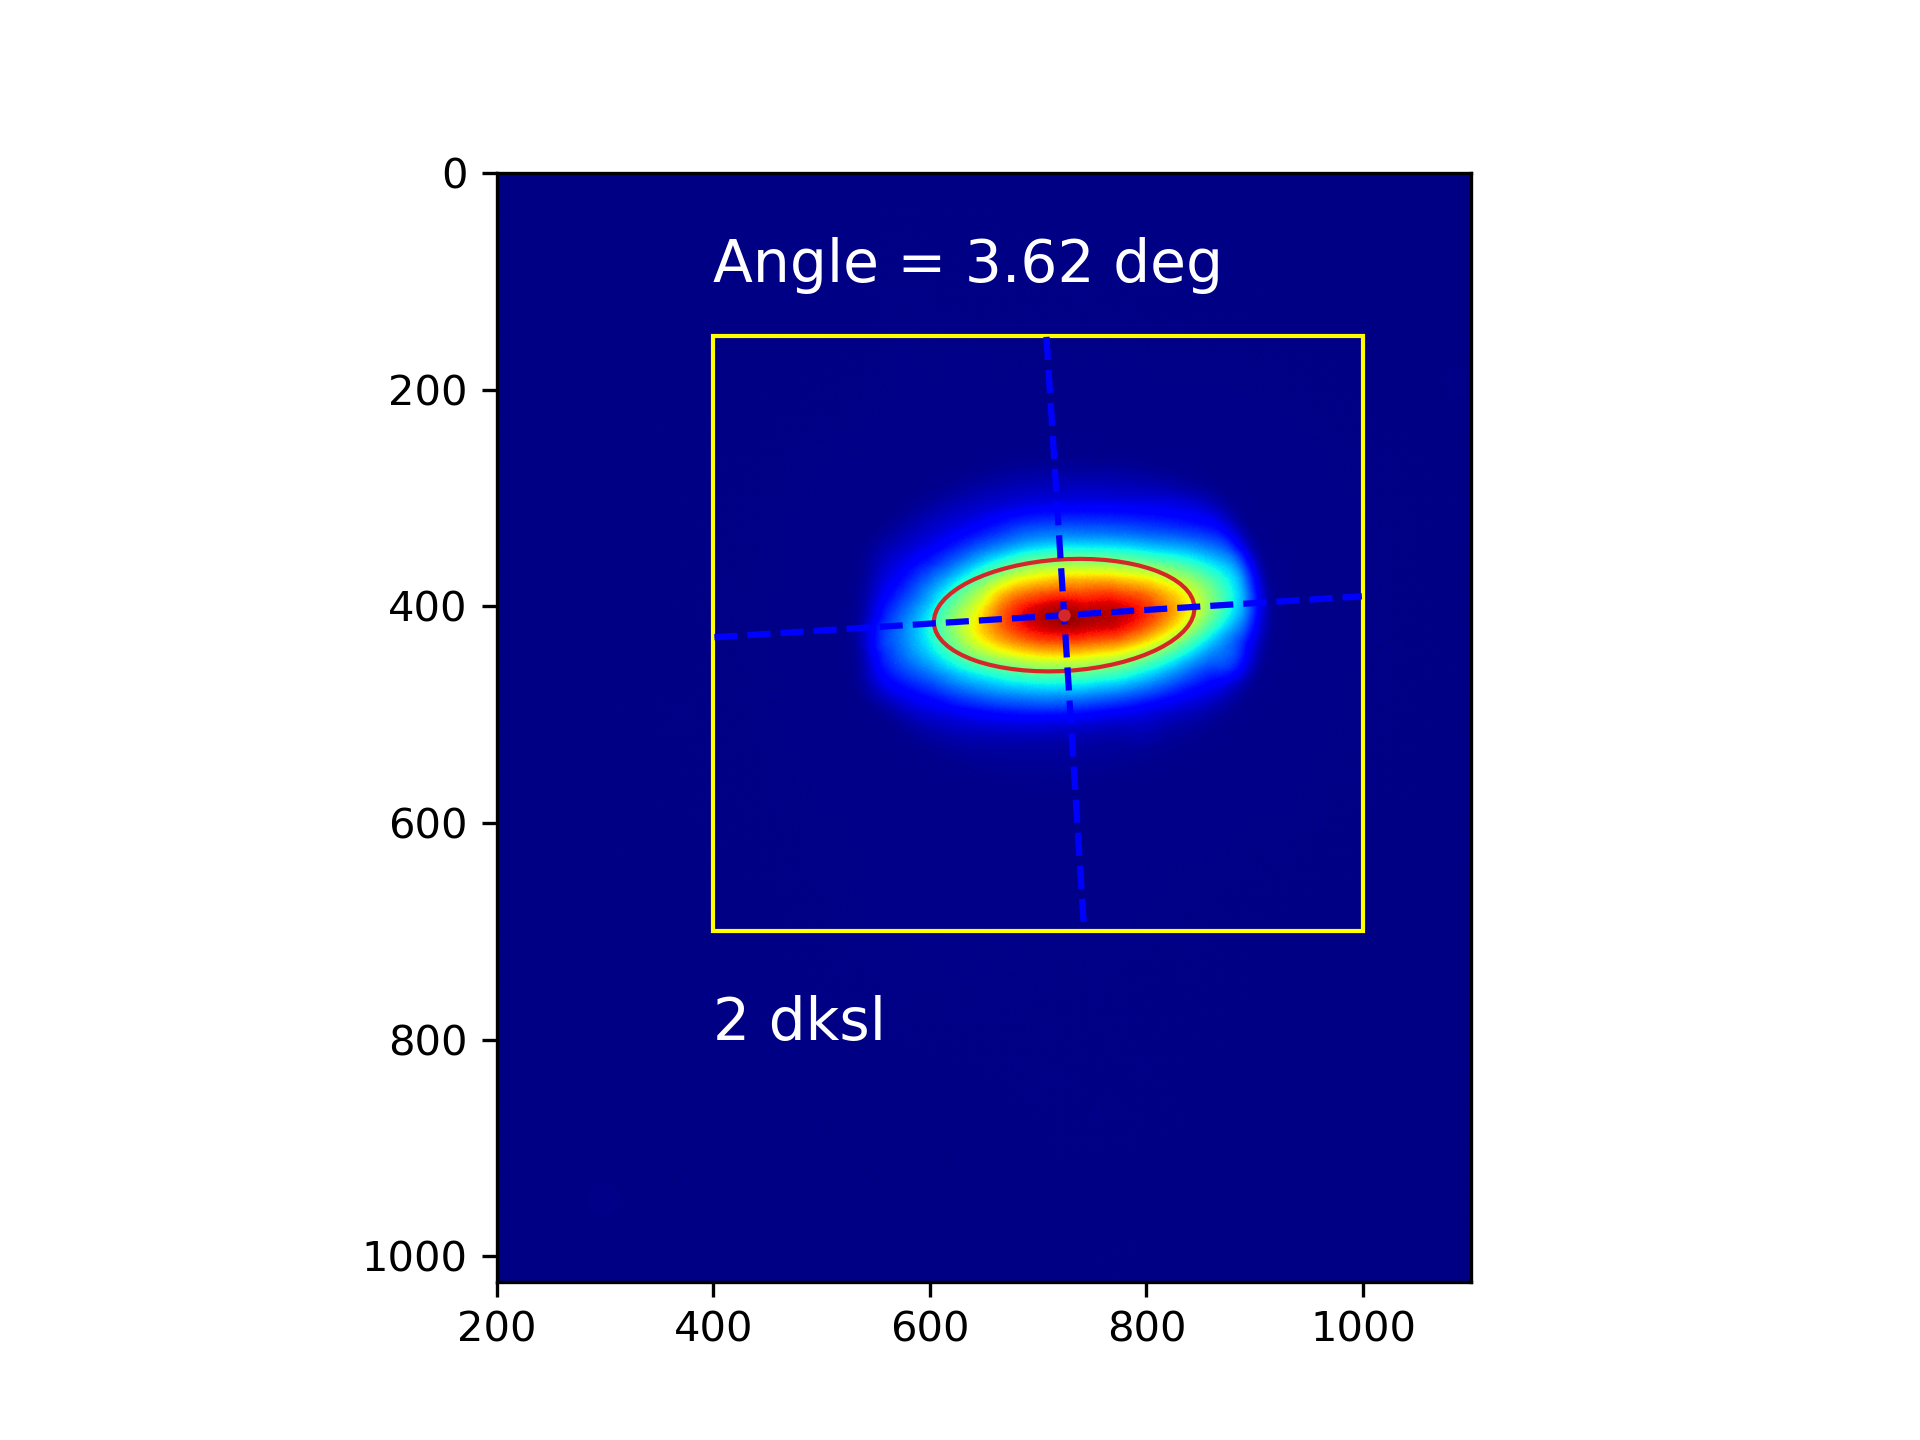
\includegraphics[width=1\linewidth, height=7cm]{2dksl_coupling_angle.png} 
\caption{Photon beam with double skew correction}
\end{subfigure}
\begin{subfigure}{0.4\textwidth}
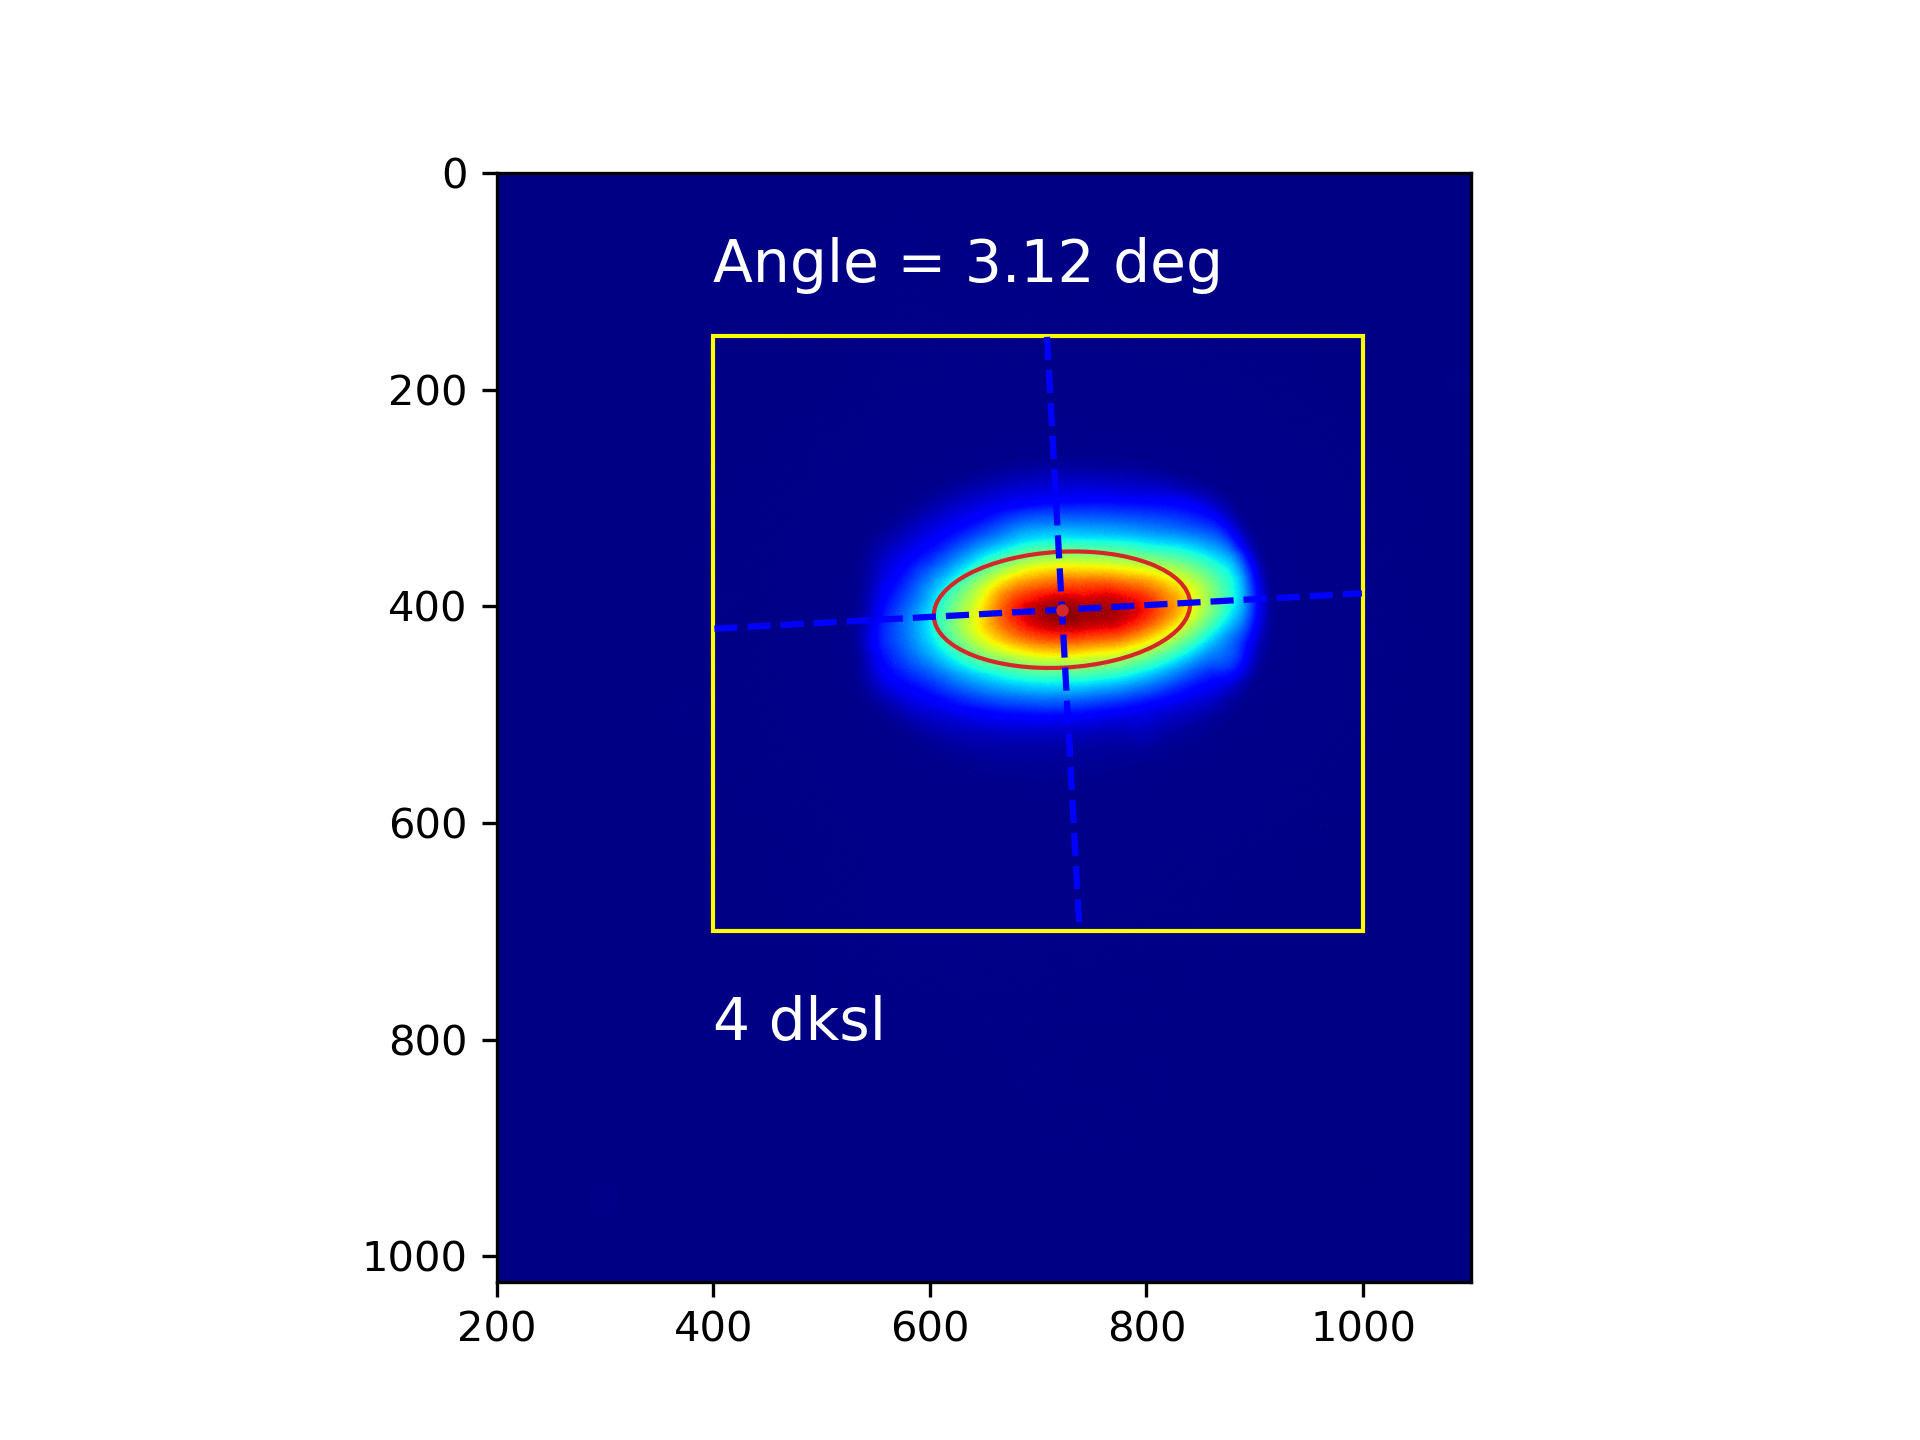
\includegraphics[width=1\linewidth, height=7cm]{4dksl_coupling_angle.png}
\caption{Photon beam with quadruple skew correction}
\end{subfigure}
\label{fig:meas_angle_2}
\end{figure}

No angle variation was observed for any skew correction.

\section{Conclusion}
\par Although an asymmetry was observed in the detuned
 photon beam, the attempt to correct the angle using skew 
 adjustments was unsuccessful. It is possible that the electron
  beam is indeed tilted in the straight section, and the algorithm
   used to calculate the skew forces may need to be revisited. A follow-up
    experiment could involve creating beam bumps to scan the entire flux density
     distribution, as even with fully open slits, the distribution remained larger
      than expected. Acquiring the full profile might provide a clearer view of the
       asymmetry.

\end{document}
